%%	SECCION documentclass																									 %%	
%%---------------------------------------------------------------------------%%
\documentclass{article}

%%---------------------------------------------------------------------------%%
%%	SECCION usepackage																											 %%	
%%---------------------------------------------------------------------------%%
\usepackage{amsmath, amsthm}
\usepackage[spanish,activeacute]{babel}
\usepackage{caratula}
\usepackage{a4wide}
\usepackage{hyperref}
\usepackage{fancyhdr}
% \usepackage{moreverb}
\usepackage{graphicx} % Para el logo magico!
\usepackage{capt-of}
\usepackage{afterpage}
\usepackage{float}
\usepackage{amssymb}
\usepackage{amsmath}
\usepackage[latin1]{inputenc}
\usepackage{subfigure}
\usepackage{algorithm}
\usepackage{algorithmic}
\usepackage[dvipsnames,usenames]{color}
\usepackage{amsfonts}
\usepackage{code_color}

%%---------------------------------------------------------------------------%%
%%	SECCION opciones																												 %%	
%%---------------------------------------------------------------------------%%
\parskip    = 11 pt
\headheight	= 13.1pt
\pagestyle	{fancy}
\definecolor{orange}{rgb}{1,0.5,0}

\addtolength{\headwidth}{1.0in}

\addtolength{\oddsidemargin}{-0.5in}
\addtolength{\textwidth}{1.0in}
\addtolength{\topmargin}{-0.8in}
\addtolength{\textheight}{0.7in}

%%%---------------------------------------------------------------------------%%
%%%	SECCION listings    													 %%	
%%%---------------------------------------------------------------------------%%
%\usepackage{listings}
%\lstset{
%		language=C++,
%		basicstyle=\ttfamily \small,
%		keepspaces=true,
%		flexiblecolumns=false,
%		basewidth={0.5em,0.45em},
%		keywordstyle=\ttfamily \bfseries \hlkwa,
%		tabsize=4
%}

%%---------------------------------------------------------------------------%%
%%	SECCION document	 %%	
%%---------------------------------------------------------------------------%%
\begin{document}
\renewcommand{\chaptername}{Parte }
\renewcommand{\algorithmicrequire}{\textcolor{blue}{\textbf{Requiere:}}}
\renewcommand{\algorithmicensure}{\textbf{Devuelve:}}
\renewcommand{\algorithmicend}{\textbf{Fin}}
\renewcommand{\algorithmicif}{\textcolor{blue}{\textbf{Si}}}
\renewcommand{\algorithmicthen}{\textcolor{blue}{}} %%\textbf{entonces}}}
\renewcommand{\algorithmicelse}{\textcolor{red}{\textbf{Si no}}}
\renewcommand{\algorithmicelsif }{\textcolor{blue}{\textbf{Si no y}}}
\renewcommand{\algorithmicendif}{\textcolor{blue}{\textbf{Fin si}}}
\renewcommand{\algorithmicfor}{\textcolor{ForestGreen}{\textbf{Para}}}
\renewcommand{\algorithmicendfor}{\textcolor{ForestGreen}{\textbf{Fin para}}}
\renewcommand{\algorithmicwhile}{\textcolor{ForestGreen}{\textbf{Mientras}}}
\renewcommand{\algorithmicendwhile}{\textcolor{ForestGreen}{\textbf{Fin mientras}}}
\renewcommand{\algorithmicdo}{\textcolor{ForestGreen}{}} %%\textbf{hacer}}}
\renewcommand{\algorithmicreturn}{\textbf{Devolver}}
\floatname{algorithm}{Algoritmo}

%%---- Caratula -------------------------------------------------------------%%
\materia{Problemas, algoritmos y programaci�n (2010)}
\titulo{Trabajo Pr'actico n� 1}


\integrante{Barenbaum, Pablo}{124/04}{pablo.barenbaum@gmail.com}
\integrante{Mart'inez, Federico}{17/06}{federicoemartinez@gmail.com}
\integrante{Sainz-Tr'apaga, Gonzalo}{454/06}{gonzalo@sainztrapaga.com.ar}
\grupo{Grupo 1}
\resumen{
El siguiente informe presenta la resoluci�n a los 4 problemas correspondientes al primer trabajo pr\'actico de la materia problemas, algoritmos y programaci�n en el primer cuatrimestre del 2010. En el mismo se encuentra la explicaci�n del algoritmo utilizado para resolver cada problema, as� como tambi�n la implementaci�n en C++ de los mismos.
}

% TOC, usa estilos locos
\maketitle
\pagestyle{empty}
{
\fancypagestyle{plain}
    {
    \fancyhead{}
    \fancyfoot{}
    \renewcommand{\headrulewidth}{0.0pt}
    } % clear header and footer of plain page because of ToC
%\tableofcontents
}

\newpage
% arreglos los estilos para el resto del documento, y
% reseteo los numeros de pagina para que queden bien
\pagenumbering{arabic}
\fancypagestyle{plain} {
    \fancyhead[LO]{Barenbaum, Mart�nez, Sainz Tr�paga}
    \fancyhead[C]{}
    \fancyhead[RO]{P\'agina \thepage\ de \pageref{LastPage}}
    \fancyfoot{}
    \renewcommand{\headrulewidth}{0.4pt}
}
\pagestyle{plain}

\section{100 - The $3n + 1$ problem}

\textbf{Problema:} dados $i$ y $j$, encontrar la longitud m\'axima del ciclo, seg\'un la sucesi\'on de Collatz, para todos los
n\'umeros entre $i$ y $j$, donde $i, j$ est\'an en el rango $[1,1\,000\,000)$.

\begin{figure}[H]
\centering
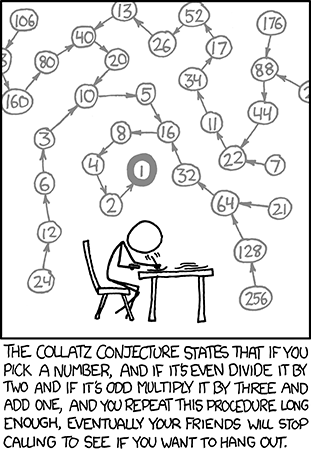
\includegraphics[scale=0.70]{./figuras/collatz_conjecture.png}
\end{figure}

\subsection{Resoluci\'on}
Para resolver este ejercicio se calculan los per\'iodos de todos los n\'umeros entre $i$ y $j$,
memorizando en un arreglo los per\'iodos ya calculados, para de esta manera no repetir c\'alculos.

Como estructura para memorizar, se utiliza un arreglo de un mill\'on de posiciones.
En general, para calcular el per\'iodo de los n\'umeros en $[1,n]$,
{\em podr\'ia} ser necesario calcular valores fuera de ese rango. La decisi\'on que tomamos fue no
memorizar el per\'iodo de los n\'umeros mayores que $999\,999$.
Ensayamos otras implementaciones que usaban un \texttt{map} para
memorizar los per\'iodos de todos los valores, pero en la pr\'actica
(adem\'as de cambiar la complejidad por usar un diccionario sobre \'arbol binario)
esto introduc\'ia un factor constante que lo hac\'ia bastante m\'as lento.

Si hubiera muchas b\'usquedas en intervalos grandes, se podr\'ia pensar en usar alguna
estructura de datos auxiliar que permitiera determinar r\'apidamente el
m\'aximo de un intervalo de un arreglo (como rmq). A modo de prueba, implementamos
una versi\'on simple de rmq (en la que una consulta cuesta $O(\sqrt{n})$), pero
el algorimo que usaba esa estructura tambi\'en resultaba comparativamente 
costoso en la pr\'actica.

%, porque usando un arreglo esto podr\'ia eventualmente necesitar una gran cantidad de memoria.
%%Es por esta raz�n que podr�a ocurrir que se repitan calculos, sin embargo creemos que el impacto que tienen esas repeticiones es despreciable.
%A la hora de realizar varias b\'usquedas, cada una se beneficia de los c\'a de periodos hechos en las anteriores. No obstante ello, si hay muchas busquedas grandes, todas recorren el rango entero. Esto podr�a hacerse de modo mas eficiente a fin de reducir el tiempo de las busquedas, sin embargo consideramos que eso escapa al problema.

Como observaci\'on adicional, se puede ver que, si $i \leq \lfloor j / 2 \rfloor$, no es
necesario buscar el m\'aximo en todo el intervalo $[i,j]$,
porque todos los valores menores que $j / 2$ tienen a su doble
dentro del intervalo. Por lo cual, dado que $periodo(2x) = periodo(x) + 1$,
el valor m\'aximo no se alcanza antes de $\lceil j / 2 \rceil$.

\begin{algorithm}[H]
\begin{algorithmic}
\caption{M\'aximo per\'iodo en un intervalo}
\PARAMS{$i,j$: bordes del intervalo donde buscar (se asume $i \leq j$)}
\ENSURE{ $maximo$: largo del per\'iodo m�ximo}
\STATE $periodo_1 := 1$
\STATE $desde := max(i,\lceil j/2 \rceil)$
\STATE $maximo := 0$
\FOR{cada $n$ entre $desde$ y $j$}
  \STATE $maximo := max(maximo, periodo_n)$
\ENDFOR
%\RETURN $maximo$
\end{algorithmic}
\end{algorithm}

\begin{algorithm}[H]
\begin{algorithmic}
\caption{Per\'iodo de un n\'umero de acuerdo con la relaci\'on de Collatz}
\PARAMS{$i$: n\'umero cuyo per\'iodo interesa conocer}
\IF{$periodo_i$ est\'a memorizado}
  \RETURN valor memorizado
\ELSE
  \STATE $p := periodo_{i'} + 1$ donde $i'$ es el siguiente de $i$ seg\'un la relaci\'on de Collatz
  \STATE memorizar $periodo_i = p$ si corresponde
  \RETURN $p$
\ENDIF
\end{algorithmic}
\end{algorithm}

Con respecto a la complejidad, si se tiene como entrada el intervalo $[i,j]$ (asumiendo
$i \leq j$), se calcula el per\'iodo de a lo sumo $j - i + 1$ n�meros. Ahora bien, $O(j-i) \subseteq O(j)$.
En muchos casos, calcular el per\'iodo requiere pocos pasos, porque alcanza con
buscar en el arreglo un per\'iodo ya calculado en otro paso; pero esto no ocurre siempre.
Sea $P$ el per\'iodo m�ximo en el intervalo sobre el que se realiza la consulta. Como cota superior
para el peor caso, calcular cada per\'iodo requiere $P$ pasos. Por esta raz\'on, la complejidad
del algoritmo es $O(P \cdot j)$.
Esta cota es bastante pesimista, ya que muy pocas veces se hacen
$P$ c\'alculos por n�mero.

%En particular, una vez que ya se calcularon todos
%los per\'iodos, las posteriores b\'usquedas requieren $O(max(i,j))$, ya que
%s\'olo se debe buscar el m\'aximo entre los valores de un arreglo.
En particular, si se realizan $n$ consultas, la complejidad, calculada
de la manera anterior, ser\'ia $O(P \cdot \sum_{k=1}^{n}{j_k})$,
donde $[i_k,j_k]$ es el intervalo de la $k$-\'esima consulta.
Pero, dado que acceder a un elemento ya memorizado es $O(1)$, el costo
del algoritmo es a lo sumo el de inicializar todo el arreglo una vez
m\'as el de buscar el m\'aximo para responder cada consulta, es
decir $O(P \cdot j_{\max} + \sum_{k=1}^{n}{j_k})$, donde $j_{\max} = \max_k{j_k}$.

En el intervalo $[1,999\,999]$ el valor de $P$ es $525$. Sin embargo, en
general, $P$ no es f\'acil de acotar. De hecho, si se pudiera acotar siempre,
se habr\'ia resuelto la conjetura de Collatz.

\subsection{Implementaci�n}

\noindent
\ttfamily
\shorthandoff{"}\\
\hlstd{}\hlline{\ 1\ }\hldir{\#include\ $<$stdio.h$>$}\\
\hlline{\ 2\ }\hlstd{}\hldir{\#include\ $<$iostream$>$}\\
\hlline{\ 3\ }\hlstd{}\hldir{\#include\ $<$vector$>$}\\
\hlline{\ 4\ }\hlstd{}\hlkwa{using\ namespace\ }\hlstd{std}\hlsym{;}\\
\hlline{\ 5\ }\hlstd{}\\
\hlline{\ 6\ }\hlkwc{typedef\ }\hlstd{}\hlkwb{unsigned\ int\ }\hlstd{uint}\hlsym{;}\\
\hlline{\ 7\ }\hlstd{}\hlkwc{typedef\ }\hlstd{}\hlkwb{unsigned\ short\ }\hlstd{ushort}\hlsym{;}\\
\hlline{\ 8\ }\hlstd{}\\
\hlline{\ 9\ }\hldir{\#define\ Max\textunderscore memo\ 1000001}\\
\hlline{10\ }\hlstd{vector}\hlsym{$<$}\hlstd{ushort}\hlsym{$>$\ }\hlstd{}\hlkwd{d}\hlstd{}\hlsym{(}\hlstd{Max\textunderscore memo}\hlsym{,\ }\hlstd{}\hlnum{0}\hlstd{}\hlsym{);}\\
\hlline{11\ }\hlstd{}\\
\hlline{12\ }\hldir{\#define\ memorizado(x)\ ((x)\ $<$\ Max\textunderscore memo\ \&\&\ d{[}(x){]}\ !=\ 0)}\\
\hlline{13\ }\hlstd{}\hldir{\#define\ next(n)\ ((n)\ \%\ 2\ ==\ 0\ ?\ (n)\ /\ 2\ :\ 3\ {*}\ (n)\ +\ 1)}\\
\hlline{14\ }\hlstd{\\
\hlline{15\ }ushort\ }\hlkwd{periodo}\hlstd{}\hlsym{(}\hlstd{uint\ n}\hlsym{)\ \{}\\
\hlline{16\ }\hlstd{\ }\hlkwa{if\ }\hlstd{}\hlsym{(}\hlstd{}\hlkwd{memorizado}\hlstd{}\hlsym{(}\hlstd{n}\hlsym{))\ \{}\\
\hlline{17\ }\hlstd{}\hlstd{\ \ }\hlstd{}\hlkwa{return\ }\hlstd{d}\hlsym{{[}}\hlstd{n}\hlsym{{]};}\\
\hlline{18\ }\hlstd{\ }\hlsym{\}\ }\hlstd{}\hlkwa{else\ }\hlstd{}\hlsym{\{}\\
\hlline{19\ }\hlstd{}\hlstd{\ \ }\hlstd{ushort\ p\ }\hlsym{=\ }\hlstd{}\hlkwd{periodo}\hlstd{}\hlsym{(}\hlstd{}\hlkwd{next}\hlstd{}\hlsym{(}\hlstd{n}\hlsym{))\ +\ }\hlstd{}\hlnum{1}\hlstd{}\hlsym{;}\\
\hlline{20\ }\hlstd{}\hlstd{\ \ }\hlstd{}\hlkwa{if\ }\hlstd{}\hlsym{(}\hlstd{n\ }\hlsym{$<$\ }\hlstd{Max\textunderscore memo}\hlsym{)\ \{}\\
\hlline{21\ }\hlstd{}\hlstd{\ \ \ }\hlstd{d}\hlsym{{[}}\hlstd{n}\hlsym{{]}\ =\ }\hlstd{p}\hlsym{;}\\
\hlline{22\ }\hlstd{}\hlstd{\ \ }\hlstd{}\hlsym{\}}\\
\hlline{23\ }\hlstd{}\hlstd{\ \ }\hlstd{}\hlkwa{return\ }\hlstd{p}\hlsym{;}\\
\hlline{24\ }\hlstd{\ }\hlsym{\}}\\
\hlline{25\ }\hlstd{}\hlsym{\}}\\
\hlline{26\ }\hlstd{\\
\hlline{27\ }ushort\ }\hlkwd{resolver}\hlstd{}\hlsym{(}\hlstd{uint\ x}\hlsym{,\ }\hlstd{uint\ y}\hlsym{)\{}\\
\hlline{28\ }\hlstd{\ ushort\ res\ }\hlsym{=\ }\hlstd{}\hlnum{0}\hlstd{}\hlsym{;}\\
\hlline{29\ }\hlstd{\ uint\ i\ }\hlsym{=\ }\hlstd{}\hlkwd{min}\hlstd{}\hlsym{(}\hlstd{x}\hlsym{,}\hlstd{y}\hlsym{);}\\
\hlline{30\ }\hlstd{\ uint\ sup\ }\hlsym{=\ }\hlstd{}\hlkwd{max}\hlstd{}\hlsym{(}\hlstd{x}\hlsym{,}\hlstd{y}\hlsym{);}\\
\hlline{31\ }\hlstd{\ ushort\ aux}\hlsym{;}\\
\hlline{32\ }\hlstd{\ i\ }\hlsym{=\ }\hlstd{}\hlkwd{max}\hlstd{}\hlsym{(}\hlstd{sup}\hlsym{/}\hlstd{}\hlnum{2}\hlstd{}\hlsym{,}\hlstd{i}\hlsym{);}\\
\hlline{33\ }\hlstd{\\
\hlline{34\ }\ }\hlkwa{while}\hlstd{}\hlsym{(}\hlstd{i\ }\hlsym{$<$=\ }\hlstd{sup}\hlsym{)\{}\\
\hlline{35\ }\hlstd{}\hlstd{\ \ }\hlstd{aux\ }\hlsym{=\ }\hlstd{}\hlkwd{periodo}\hlstd{}\hlsym{(}\hlstd{i}\hlsym{);}\\
\hlline{36\ }\hlstd{}\hlstd{\ \ }\hlstd{}\hlkwa{if\ }\hlstd{}\hlsym{(}\hlstd{aux\ }\hlsym{$>$\ }\hlstd{res}\hlsym{)\{}\\
\hlline{37\ }\hlstd{}\hlstd{\ \ \ }\hlstd{res\ }\hlsym{=\ }\hlstd{aux}\hlsym{;}\\
\hlline{38\ }\hlstd{}\hlstd{\ \ }\hlstd{}\hlsym{\}}\\
\hlline{39\ }\hlstd{}\hlstd{\ \ }\hlstd{i}\hlsym{++;}\\
\hlline{40\ }\hlstd{\ }\hlsym{\}}\\
\hlline{41\ }\hlstd{\ }\hlkwa{return\ }\hlstd{res}\hlsym{;}\\
\hlline{42\ }\hlstd{}\hlsym{\}}\\
\hlline{43\ }\hlstd{}\\
\hlline{44\ }\hlkwb{int\ }\hlstd{}\hlkwd{main}\hlstd{}\hlsym{(}\hlstd{}\hlkwb{int\ }\hlstd{argc}\hlsym{,\ }\hlstd{}\hlkwb{char\ }\hlstd{}\hlsym{{*}{*}}\hlstd{argv}\hlsym{)}\\
\hlline{45\ }\hlstd{}\hlsym{\{}\\
\hlline{46\ }\hlstd{\ uint\ x}\hlsym{,\ }\hlstd{y}\hlsym{;}\\
\hlline{47\ }\hlstd{\ d}\hlsym{{[}}\hlstd{}\hlnum{1}\hlstd{}\hlsym{{]}\ =\ }\hlstd{}\hlnum{1}\hlstd{}\hlsym{;}\\
\hlline{48\ }\hlstd{\ }\hlkwa{while\ }\hlstd{}\hlsym{(}\hlstd{}\hlkwd{scanf}\hlstd{}\hlsym{(}\hlstd{}\hlstr{"\%u\ \%u"}\hlstd{}\hlsym{,\&}\hlstd{x}\hlsym{,\&}\hlstd{y}\hlsym{)==}\hlstd{}\hlnum{2}\hlstd{}\hlsym{)\ \{}\\
\hlline{49\ }\hlstd{}\hlstd{\ \ }\hlstd{cout\ }\hlsym{$<$$<$\ }\hlstd{x\ }\hlsym{$<$$<$}\hlstd{}\hlstr{"\ "}\hlstd{}\hlsym{$<$$<$\ }\hlstd{y\ }\hlsym{$<$$<$}\hlstd{}\hlstr{"\ "}\hlstd{\ }\hlsym{$<$$<$\ }\hlstd{}\hlkwd{resolver}\hlstd{}\hlsym{(}\hlstd{x}\hlsym{,\ }\hlstd{y}\hlsym{)\ $<$$<$\ }\hlstd{endl}\hlsym{;}\\
\hlline{50\ }\hlstd{\ }\hlsym{\}}\\
\hlline{51\ }\hlstd{\ }\hlkwa{return\ }\hlstd{}\hlnum{0}\hlstd{}\hlsym{;}\\
\hlline{52\ }\hlstd{}\hlsym{\}}\\
\hlline{53\ }\hlstd{}\\
\mbox{}
\normalfont
\shorthandon{"}



\newpage
\section{861 - Little bishops}

\textbf{Problema:} dados dos enteros $n$ y $k$, devolver la cantidad
de formas de ubicar $k$ alfiles en un tablero de $n \times n$, de manera tal
que ninguno de ellos sea atacado por otro.

\subsection{Resoluci\'on}
Para resolverlo, primero notamos que las casillas negras y las blancas
son independientes, en el sentido de que un alfil en una casilla de un color
nunca puede atacar a un alfil en una casilla del color opuesto.
Por esta raz\'on, la cantidad de formas de ubicar $k$ alfiles
en un tablero de $n \times n$ se puede calcular de la siguiente manera:

Sea $a_k$ la cantidad de formas de ubicar $k$ alfiles sin que se ataquen
en un tablero de $n \times n$. Si $a_k^B$ es la cantidad de formas de ubicar 
$k$ alfiles sin que se ataquen en las casillas blancas y
$a_k^N$ es la cantidad de formas de hacerlo en las negras, entonces vale que:

$$a_k = \sum_{i=0}^k{a_i^N \cdot a_{k-i}^B}$$

Por otro lado, mirando s\'olo las casillas negras 
(es an\'alogo para las blancas) y rotando el tablero $45�$, 
el problema de ubicar alfiles se puede interpretar como un
problema de ubicar torres.

\begin{figure}[H]
\centering
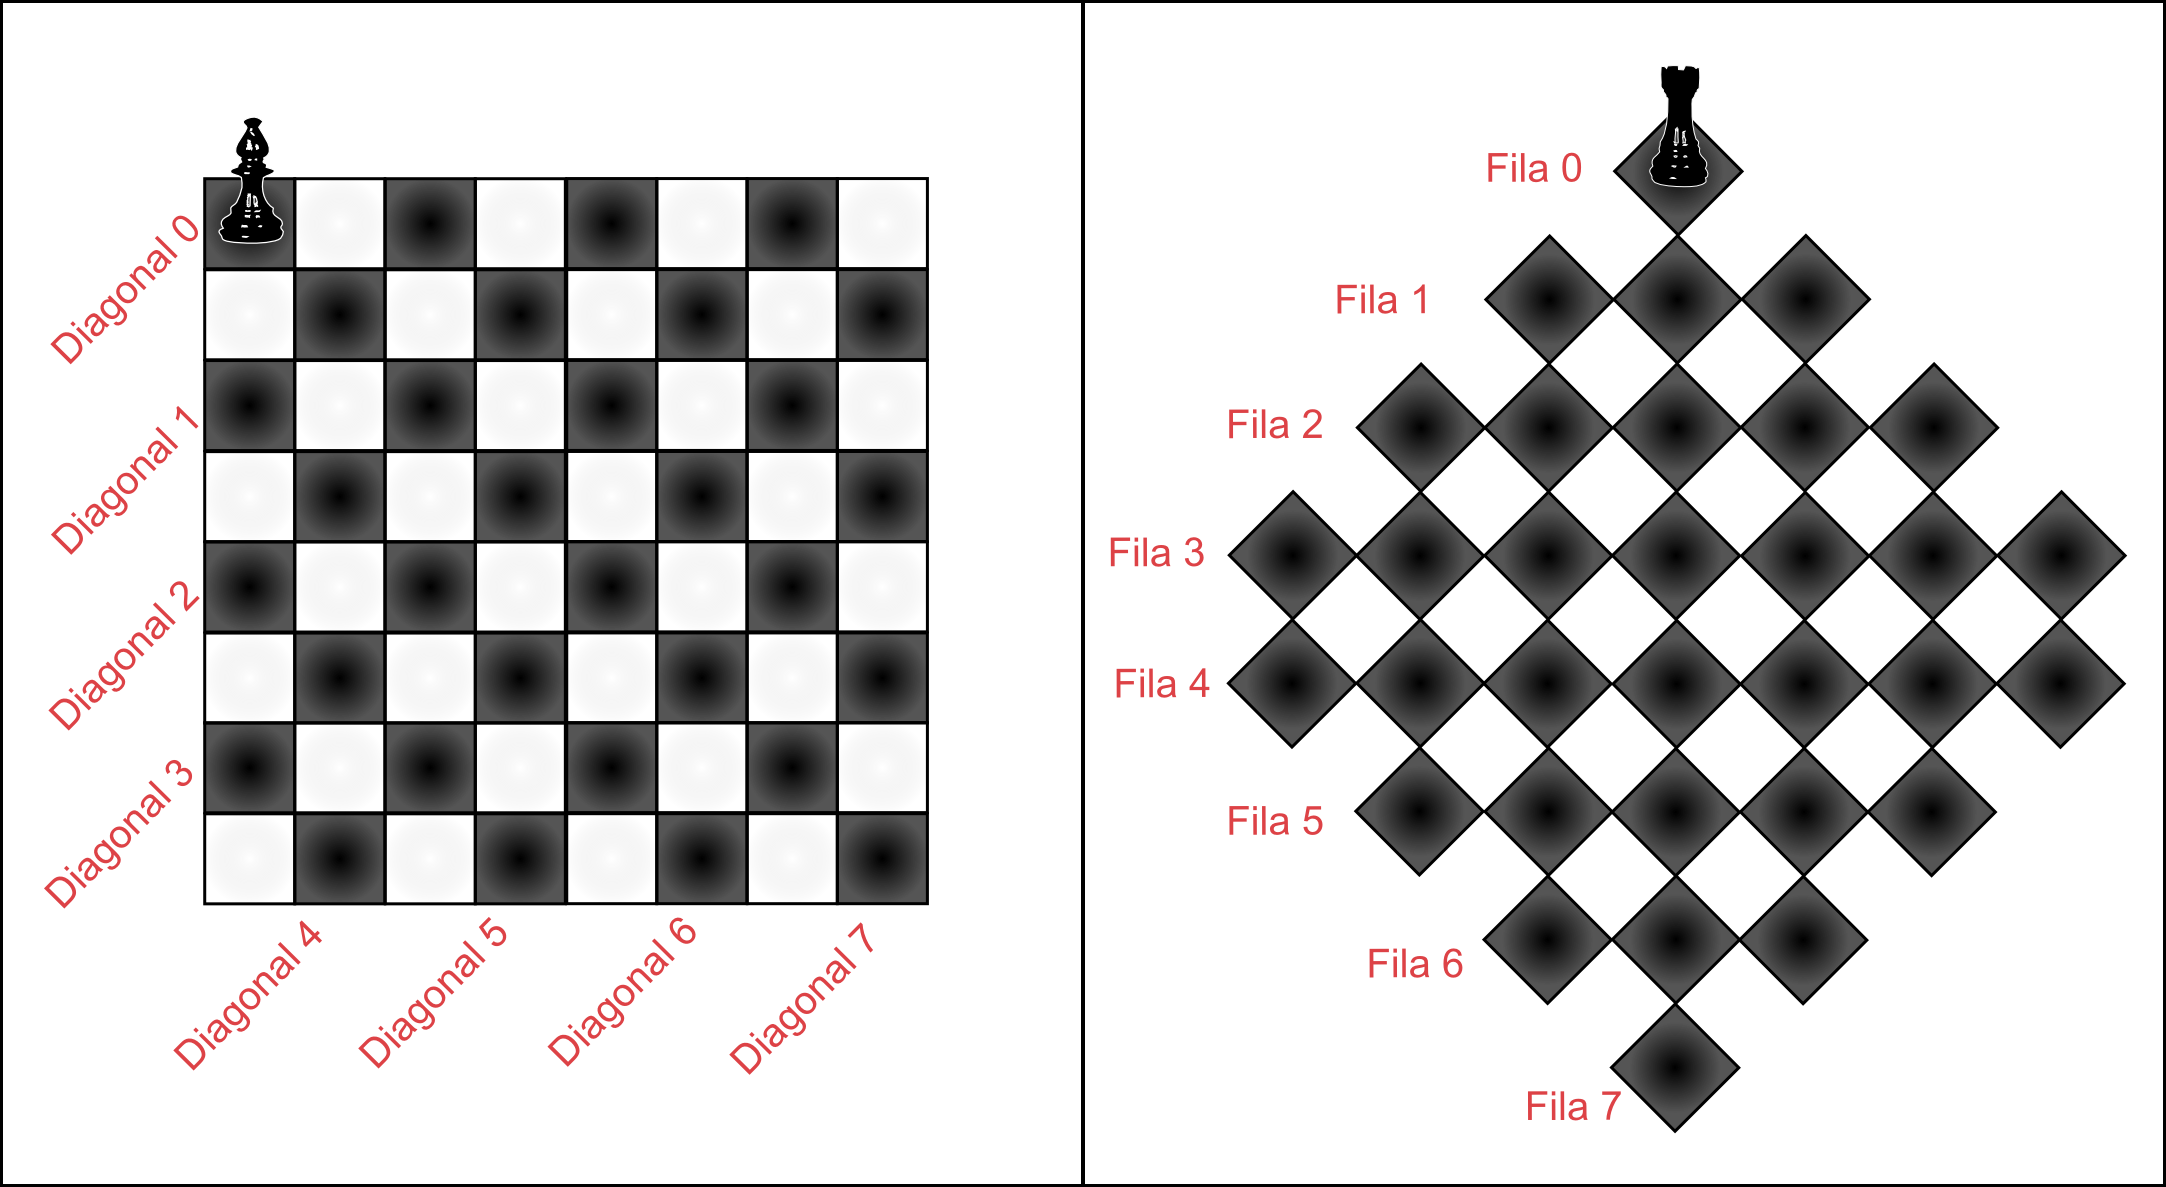
\includegraphics[scale=0.30]{./figuras/tablero1.png}
\caption{Interpretaci\'on del problema de los alfiles como uno de torres}
\end{figure}

Consideramos ahora el problema de ubicar torres, sin que se ataquen,
en un tablero de varias filas, cada una de las cuales puede tener un
n\'umero diferente de columnas.
Es f\'acil ver que a lo sumo puede haber una torre por fila, y que
permutar filas no modifica la cantidad de torres que se pueden ubicar. 
Sea $columnas(i)$ la cantidad de columnas de la fila $i$.
Si se ordenan las filas crecientemente por su cantidad de columnas,
vale que las columnas de cada fila 
est�n incluidas en las de las filas que est�n abajo. Esto quiere 
decir que, al ubicar una torre, la columna en la que fue ubicada queda
inutilizable para las filas siguientes.

A partir de esto podemos definir la siguiente recurrencia:

Sea $cantidad(i,j)=$ cantidad de formas de poner $j$ torres usando las 
primeras $i$ filas (ordenadas crecientemente por cantidad de columnas). Vale entonces 
que:

$cantidad(i,0) = 1 $, porque hay solo una forma de no poner ninguna torre.

$cantidad(0,j) = 0  \ si \ j > 0$, porque no hay forma de poner alguna torre si no quedan casillas.
 
$cantidad(i,j) = cantidad(i-1,j) + cantidad(i-1,j-1) \cdot (columnas(i)-(j-1))\ si \ i > 0$, 
porque o bien se ponen las $j$ torres en la filas anteriores, o bien se pone una en 
la fila actual y el resto en las anteriores. Al hacer eso, se est\'an ocupando $j-1$ 
columnas; las restantes quedan libres, por lo cual para cada posible forma de ubicar 
las torres en las anteriores filas hay $columnas(i) - (j-1)$ columnas libres que 
pueden usarse.

Aplicamos la resoluci\'on del problema de ubicar torres sobre las diagonales
negras y las diagonales blancas, para as\'i calcular $a^N_k$ y $a^B_k$.
Pueden hacerse las siguientes optimizaciones:
\begin{itemize}
\item No es necesario ``ordenar'' las diagonales, basta con notar que para las
casillas negras las longitudes de las diagonales son 1, 1, 3, 3, ..., etc. (para
las casillas blancas es similar pero empezando desde 2).

\item Si $n$ es par, las casillas blancas y las negras son sim\'etricas,
por lo cual la cantidad de formas de ubicar las piezas es la misma para
unas y otras (es decir, $a^B_k = a^N_k$). En ese caso, basta con resolver
el problema para las casillas de uno de los colores.

\item Si $n > 1$, la cantidad m\'axima de alfiles que se pueden poner en un tablero de $n \times n$ es $2n - 2$.
Esto es porque hay $2n - 1$ diagonales pero adem\'as no pueden ubicarse dos alfiles en esquinas opuestas\footnote{
Adem\'as est\'a demostrado: 

Dudeney, H. E. ``Bishops--Unguarded'' and ``Bishops--Guarded.'' \S 297 and 298 in Amusements in Mathematics. New York: Dover, pp. 88-89 and 96, 1970.

Madachy, J. Madachy's Mathematical Recreations. New York: Dover, pp. 36-46, 1979. }
con lo cual si el $k$ ingresado es mayor, se puede devolver 0 sin procesar nada.

\item En todas las diagonales de un color, se pueden poner a lo sumo $n - 1$ alfiles, esto es f�cil de ver, si consideramos un tablero ubicado como el de la figura, las casillas negras tienen $n$ diagonales ascendentes, pero dos son de una sola casilla y est�n en la misma diagonal descendente. Si $n$ es par las casillas blancas son sim�tricas a las negras, por lo que la cantidad de alfiles que se pueden ubicar es la misma. Si en cambio $n$ es impar, hay $n-1$ diagonales blancas ascendentes, que a lo sumo pueden tener un alfil cada una.
Es por esta raz�n que no hace falta hacer la sumatoria desde $0$ hasta $k$, sino que se puede hacer
desde $max(0, k - (n - 1))$ hasta $min(k, n - 1)$. Esto s\'olo vale si $n > 1$, ya que con $n = 1$
no hay casillas blancas.
\end{itemize}

En base a la recurrencia planteada, se ve que basta con llenar una matriz $M$ de $(n + 1) \times (k + 1)$
para las negras y otra para las blancas, de modo que $M[i][j]=cantidad(i,j)$. El siguiente es el
algoritmo de llenado de la tabla para las casillas negras. Si el tablero es impar, el algoritmo
para las casillas blancas es similar. Dado que en cada paso s\'olo se necesita la fila anterior,
en la implementaci\'on la matriz se representa guardando s\'olo las \'ultimas dos filas,
cada una de $k + 1$ elementos.

\begin{algorithm}[H]
\begin{algorithmic}
\caption{\texttt{ubicar\_en\_negras}: maneras de ubicar $\leq k$ alfiles en las casillas negras de un tablero de $n \times n$}
\PARAMS{$n$: alto del tablero, $k$: m\'axima cantidad de alfiles que se quieren poner}
\STATE $M$ := matriz de $(n + 1)$ filas y  $(k+1)$ columnas %%tal que $M_{ij}=0$
%\STATE\COMMENT{$M_{i,j}$ = cantidad de maneras de poner $j$ alfiles en las diagonales negras $[0,i)$}
\STATE $M_{i,0} := 1$ para todo $i$
\STATE $M_{0,j} := 0$ para todo $j > 0$
\FOR{cada $i$ en $[1,n]$}
	\STATE $casillas$ := n\'umero de casillas de la $(i - 1)$-\'esima diagonal negra
	\FOR{cada $j$ en $[1,k]$}
		\STATE $M_{i,j} := M_{i-1,j} + M_{i-1,j-1}*(casillas - (j-1))$
	\ENDFOR
\ENDFOR
\STATE $resultado := M[n]$ \COMMENT{\'ultima fila de la matriz}
\RETURN $resultado$ \COMMENT{$resultado[j] = $ cantidad de maneras de poner $j$ alfiles en las casillas negras del tablero}
\end{algorithmic}
\end{algorithm}

\begin{algorithm}[H]
\begin{algorithmic}
\caption{Maneras de ubicar $k$ alfiles en un tablero de $n \times n$}
\PARAMS{$n$: alto del tablero, $k$: cantidad de alfiles que se quieren poner}
\STATE Si $k=0$ devolver 1.
\STATE Si el tablero es s\'olo una casilla y $k=1$, devolver 1.
\STATE Si $k >$ m\'aximo numero de alfiles en un tablero de $n \times n$ devolver 0.
\STATE $negras :=$ \texttt{ubicar\_en\_negras($n$, $k$)}
\STATE $blancas :=$ si $n$ es par, es igual a $negras$; si no, \texttt{ubicar\_en\_blancas($n$, $k$)}
\STATE $maneras := 0$
\STATE $inf := max(k - (n - 1), 0)$
\STATE $sup := min(k, n - 1) + 1$
\FOR{cada $a$ en [$inf$, $sup$]}
		\STATE $maneras := maneras + negras_a * blancas_{k - a}$
\ENDFOR
\RETURN $maneras$
\end{algorithmic}
\end{algorithm}

Con respecto a la complejidad, vimos que si $k > 2n-2$ no es necesario calcular
la matriz. Esto se puede ver en $O(1)$. %Si $k <= 2n-2$ entonces tenemos que contar.
Por lo tanto, para calcular la complejidad del resto del algoritmo, se
puede asumir que $k \in O(n)$.

Computar cada matriz toma $O(n \cdot k)$, que es $O(n^2)$. A lo sumo se computan
dos matrices. El costo de recorrer las \'ultimas filas y hacer el producto es
$O(k)$, que nuevamente es $O(n)$. Por lo tanto, la complejidad temporal en peor caso
es $O(n^2)$.

En cuanto a la memoria, alcanza con guardar las \'ultimas dos filas de la matriz
en cada paso, por lo cual es la complejidad es $O(k)$ que es $O(n)$.

\subsection{Implementaci�n}

\noindent
\ttfamily
\shorthandoff{"}\\
\hlstd{}\hlline{\ 1\ }\hldir{\#include\ $<$iostream$>$}\\
\hlline{\ 2\ }\hlstd{}\hldir{\#include\ $<$vector$>$}\\
\hlline{\ 3\ }\hlstd{}\\
\hlline{\ 4\ }\hlkwa{using\ namespace\ }\hlstd{std}\hlsym{;}\\
\hlline{\ 5\ }\hlstd{}\\
\hlline{\ 6\ }\hlkwc{typedef\ }\hlstd{}\hlkwb{unsigned\ int\ }\hlstd{uint}\hlsym{;}\\
\hlline{\ 7\ }\hlstd{}\hlkwc{typedef\ }\hlstd{}\hlkwb{unsigned\ long\ long\ int\ }\hlstd{uint64}\hlsym{;}\\
\hlline{\ 8\ }\hlstd{}\\
\hlline{\ 9\ }\hldir{\#define\ forsn(i,\ s,\ n)}\hlstd{\ \ }\hldir{for\ (uint\ i\ =\ (s);\ i\ $<$\ (n);\ i++)}\\
\hlline{10\ }\hlstd{}\hldir{\#define\ forn(i,\ n)}\hlstd{\ \ }\hldir{forsn\ (i,\ 0,\ n)}\\
\hlline{11\ }\hlstd{}\\
\hlline{12\ }\hldir{\#define\ num\textunderscore diagonals(n)\ (2\ {*}\ (n)\ {-}\ 1)}\\
\hlline{13\ }\hlstd{}\\
\hlline{14\ }\hlkwc{typedef\ }\hlstd{vector}\hlsym{$<$}\hlstd{uint64}\hlsym{$>$\ }\hlstd{vuint64}\hlsym{;}\\
\hlline{15\ }\hlstd{}\hlkwc{typedef\ }\hlstd{vector}\hlsym{$<$}\hlstd{vuint64}\hlsym{$>$\ }\hlstd{vvuint64}\hlsym{;}\\
\hlline{16\ }\hlstd{}\\
\hlline{17\ }\hldir{\#define\ BLACK\ 0}\\
\hlline{18\ }\hlstd{}\hldir{\#define\ WHITE\ 1}\\
\hlline{19\ }\hlstd{}\hlslc{//\ m:\ output\ matrix,\ should\ have\ 2\ rows\ and\ k\ +\ 1\ columns}\\
\hlline{20\ }\hlstd{}\hlslc{//\ black\textunderscore white\ ==\ 1\ iff\ we\ are\ dealing\ with\ the\ white\ cells\ and\ an\ odd\ value\ of\ n\ }\\
\hlline{21\ }\hlstd{vuint64\ }\hlsym{{*}}\hlstd{}\hlkwd{put\textunderscore bishops\textunderscore monochrome}\hlstd{}\hlsym{(}\hlstd{uint\ n}\hlsym{,\ }\hlstd{uint\ k}\hlsym{,\ }\hlstd{}\hlkwb{bool\ }\hlstd{black\textunderscore white}\hlsym{,\ }\hlstd{vvuint64}\hlsym{\&\ }\hlstd{m}\hlsym{)\ \{}\\
\hlline{22\ }\hlstd{\ }\hlkwb{bool\ }\hlstd{row\ }\hlsym{=\ }\hlstd{}\hlnum{0}\hlstd{}\hlsym{;}\\
\hlline{23\ }\hlstd{\\
\hlline{24\ }\ m}\hlsym{{[}}\hlstd{}\hlnum{0}\hlstd{}\hlsym{{]}{[}}\hlstd{}\hlnum{0}\hlstd{}\hlsym{{]}\ =\ }\hlstd{}\hlnum{1}\hlstd{}\hlsym{;\ }\hlstd{}\hlslc{//\ we\ can\ always\ put\ 0\ bishops}\\
\hlline{25\ }\hlstd{\ m}\hlsym{{[}}\hlstd{}\hlnum{1}\hlstd{}\hlsym{{]}{[}}\hlstd{}\hlnum{0}\hlstd{}\hlsym{{]}\ =\ }\hlstd{}\hlnum{1}\hlstd{}\hlsym{;}\\
\hlline{26\ }\hlstd{\ \\
\hlline{27\ }\ }\hlkwd{forn\ }\hlstd{}\hlsym{(}\hlstd{i}\hlsym{,\ }\hlstd{n\ }\hlsym{{-}\ }\hlstd{black\textunderscore white}\hlsym{)\ \{}\\
\hlline{28\ }\hlstd{}\hlstd{\ \ }\hlstd{uint\ num\textunderscore cells\ }\hlsym{=\ }\hlstd{}\hlnum{2\ }\hlstd{}\hlsym{{*}\ (}\hlstd{i\ }\hlsym{/\ }\hlstd{}\hlnum{2}\hlstd{}\hlsym{)\ +\ }\hlstd{}\hlnum{1\ }\hlstd{}\hlsym{+\ }\hlstd{black\textunderscore white}\hlsym{;}\\
\hlline{29\ }\hlstd{}\hlstd{\ \ }\hlstd{}\hlkwd{forsn\ }\hlstd{}\hlsym{(}\hlstd{j}\hlsym{,\ }\hlstd{}\hlnum{1}\hlstd{}\hlsym{,\ }\hlstd{k\ }\hlsym{+\ }\hlstd{}\hlnum{1}\hlstd{}\hlsym{)\ \{}\\
\hlline{30\ }\hlstd{}\hlstd{\ \ \ }\hlstd{m}\hlsym{{[}}\hlstd{row}\hlsym{{]}{[}}\hlstd{j}\hlsym{{]}\ =\ }\hlstd{m}\hlsym{{[}!}\hlstd{row}\hlsym{{]}{[}}\hlstd{j}\hlsym{{]}\ +\ }\hlstd{m}\hlsym{{[}!}\hlstd{row}\hlsym{{]}{[}}\hlstd{j\ }\hlsym{{-}\ }\hlstd{}\hlnum{1}\hlstd{}\hlsym{{]}\ {*}\ (}\hlstd{num\textunderscore cells\ }\hlsym{{-}\ (}\hlstd{j\ }\hlsym{{-}\ }\hlstd{}\hlnum{1}\hlstd{}\hlsym{));}\\
\hlline{31\ }\hlstd{}\hlstd{\ \ }\hlstd{}\hlsym{\}}\\
\hlline{32\ }\hlstd{}\hlstd{\ \ }\hlstd{row\ }\hlsym{=\ !}\hlstd{row}\hlsym{;}\\
\hlline{33\ }\hlstd{\ }\hlsym{\}}\\
\hlline{34\ }\hlstd{\ }\hlkwa{return\ }\hlstd{}\hlsym{\&}\hlstd{m}\hlsym{{[}!}\hlstd{row}\hlsym{{]};}\\
\hlline{35\ }\hlstd{}\hlsym{\}}\\
\hlline{36\ }\hlstd{\\
\hlline{37\ }uint64\ }\hlkwd{put\textunderscore bishops}\hlstd{}\hlsym{(}\hlstd{uint\ n}\hlsym{,\ }\hlstd{uint\ k}\hlsym{)\ \{}\\
\hlline{38\ }\hlstd{\ }\hlkwa{if\ }\hlstd{}\hlsym{(}\hlstd{k\ }\hlsym{==\ }\hlstd{}\hlnum{0}\hlstd{}\hlsym{)\ }\hlstd{}\hlkwa{return\ }\hlstd{}\hlnum{1}\hlstd{}\hlsym{;}\\
\hlline{39\ }\hlstd{\ }\hlkwa{if\ }\hlstd{}\hlsym{(}\hlstd{k\ }\hlsym{==\ }\hlstd{}\hlnum{1\ }\hlstd{}\hlsym{\&\&\ }\hlstd{n\ }\hlsym{==\ }\hlstd{}\hlnum{1}\hlstd{}\hlsym{)\ }\hlstd{}\hlkwa{return\ }\hlstd{}\hlnum{1}\hlstd{}\hlsym{;}\\
\hlline{40\ }\hlstd{\ }\hlkwa{if\ }\hlstd{}\hlsym{(}\hlstd{k\ }\hlsym{$>$\ }\hlstd{}\hlkwd{num\textunderscore diagonals}\hlstd{}\hlsym{(}\hlstd{n}\hlsym{)\ {-}\ }\hlstd{}\hlnum{1}\hlstd{}\hlsym{)\ }\hlstd{}\hlkwa{return\ }\hlstd{}\hlnum{0}\hlstd{}\hlsym{;}\\
\hlline{41\ }\hlstd{\\
\hlline{42\ }\ vvuint64\ }\hlkwd{matrix\textunderscore black}\hlstd{}\hlsym{(}\hlstd{}\hlnum{2}\hlstd{}\hlsym{,\ }\hlstd{}\hlkwd{vuint64}\hlstd{}\hlsym{(}\hlstd{k\ }\hlsym{+\ }\hlstd{}\hlnum{1}\hlstd{}\hlsym{,\ }\hlstd{}\hlnum{0}\hlstd{}\hlsym{));}\\
\hlline{43\ }\hlstd{\ vvuint64\ }\hlkwd{matrix\textunderscore white}\hlstd{}\hlsym{(}\hlstd{}\hlnum{2}\hlstd{}\hlsym{,\ }\hlstd{}\hlkwd{vuint64}\hlstd{}\hlsym{(}\hlstd{k\ }\hlsym{+\ }\hlstd{}\hlnum{1}\hlstd{}\hlsym{,\ }\hlstd{}\hlnum{0}\hlstd{}\hlsym{));}\\
\hlline{44\ }\hlstd{\\
\hlline{45\ }\ vuint64}\hlsym{\&\ }\hlstd{}\hlkwd{black}\hlstd{}\hlsym{({*}}\hlstd{}\hlkwd{put\textunderscore bishops\textunderscore monochrome}\hlstd{}\hlsym{(}\hlstd{n}\hlsym{,\ }\hlstd{k}\hlsym{,\ }\hlstd{BLACK}\hlsym{,\ }\hlstd{matrix\textunderscore black}\hlsym{));}\\
\hlline{46\ }\hlstd{\ vuint64}\hlsym{\&\ }\hlstd{}\hlkwd{white}\hlstd{}\hlsym{(}\hlstd{n\ }\hlsym{\%\ }\hlstd{}\hlnum{2\ }\hlstd{}\hlsym{==\ }\hlstd{}\hlnum{0\ }\hlstd{?\ black\ }\hlsym{:\ {*}}\hlstd{}\hlkwd{put\textunderscore bishops\textunderscore monochrome}\hlstd{}\hlsym{(}\hlstd{n}\hlsym{,\ }\hlstd{k}\hlsym{,\ }\hlstd{WHITE}\hlsym{,\ }\hlstd{matrix\textunderscore white}\hlsym{));}\\
\hlline{47\ }\hlstd{\\
\hlline{48\ }\ uint64\ ways\ }\hlsym{=\ }\hlstd{}\hlnum{0}\hlstd{}\hlsym{;}\\
\hlline{49\ }\hlstd{\ uint\ lower\ }\hlsym{=\ }\hlstd{k\ }\hlsym{$>$\ (}\hlstd{n\ }\hlsym{{-}\ }\hlstd{}\hlnum{1}\hlstd{}\hlsym{)\ }\hlstd{?\ k\ }\hlsym{{-}\ (}\hlstd{n\ }\hlsym{{-}\ }\hlstd{}\hlnum{1}\hlstd{}\hlsym{)\ :\ }\hlstd{}\hlnum{0}\hlstd{}\hlsym{;}\\
\hlline{50\ }\hlstd{\ uint\ upper\ }\hlsym{=\ }\hlstd{}\hlkwd{min}\hlstd{}\hlsym{(}\hlstd{k}\hlsym{,\ }\hlstd{n\ }\hlsym{{-}\ }\hlstd{}\hlnum{1}\hlstd{}\hlsym{)\ +\ }\hlstd{}\hlnum{1}\hlstd{}\hlsym{;}\\
\hlline{51\ }\hlstd{\ }\hlkwd{forsn\ }\hlstd{}\hlsym{(}\hlstd{a}\hlsym{,\ }\hlstd{lower}\hlsym{,\ }\hlstd{upper}\hlsym{)\ \{}\\
\hlline{52\ }\hlstd{}\hlstd{\ \ }\hlstd{ways\ }\hlsym{+=\ }\hlstd{black}\hlsym{{[}}\hlstd{a}\hlsym{{]}\ {*}\ }\hlstd{white}\hlsym{{[}}\hlstd{k\ }\hlsym{{-}\ }\hlstd{a}\hlsym{{]};}\\
\hlline{53\ }\hlstd{\ }\hlsym{\}}\\
\hlline{54\ }\hlstd{\ }\hlkwa{return\ }\hlstd{ways}\hlsym{;}\\
\hlline{55\ }\hlstd{}\hlsym{\}}\\
\hlline{56\ }\hlstd{}\\
\hlline{57\ }\hlkwb{int\ }\hlstd{}\hlkwd{main}\hlstd{}\hlsym{()\ \{}\\
\hlline{58\ }\hlstd{\ uint\ n}\hlsym{,\ }\hlstd{k}\hlsym{;}\\
\hlline{59\ }\hlstd{\ }\hlkwa{while\ }\hlstd{}\hlsym{(}\hlstd{}\hlkwa{true}\hlstd{}\hlsym{)\ \{}\\
\hlline{60\ }\hlstd{}\hlstd{\ \ }\hlstd{}\hlkwd{scanf}\hlstd{}\hlsym{(}\hlstd{}\hlstr{"\%u\ \%u"}\hlstd{}\hlsym{,\ \&}\hlstd{n}\hlsym{,\ \&}\hlstd{k}\hlsym{);}\\
\hlline{61\ }\hlstd{}\hlstd{\ \ }\hlstd{}\hlkwa{if\ }\hlstd{}\hlsym{(}\hlstd{n\ }\hlsym{==\ }\hlstd{}\hlnum{0\ }\hlstd{}\hlsym{\&\&\ }\hlstd{k\ }\hlsym{==\ }\hlstd{}\hlnum{0}\hlstd{}\hlsym{)\ }\hlstd{}\hlkwa{break}\hlstd{}\hlsym{;}\\
\hlline{62\ }\hlstd{}\hlstd{\ \ }\hlstd{cout\ }\hlsym{$<$$<$\ }\hlstd{}\hlkwd{put\textunderscore bishops}\hlstd{}\hlsym{(}\hlstd{n}\hlsym{,\ }\hlstd{k}\hlsym{)\ $<$$<$\ }\hlstd{endl}\hlsym{;}\\
\hlline{63\ }\hlstd{\ }\hlsym{\}}\\
\hlline{64\ }\hlstd{\ }\hlkwa{return\ }\hlstd{}\hlnum{0}\hlstd{}\hlsym{;}\\
\hlline{65\ }\hlstd{}\hlsym{\}}\\
\hlline{66\ }\hlstd{}\\
\mbox{}
\normalfont
\shorthandon{"}



\newpage
\section{10020 - Minimal coverage}

\textbf{Problema:} dado un conjunto de intervalos $[L_i,R_i)$, determinar
un subconjunto que cubra el segmento $[0,M)$ y que sea m\'inimo
(en el sentido de cardinalidad). En el enunciado los intervalos
se notan $[L,R]$, pero como los extremos son enteros y hay que
cubrir intervalos reales, los problemas son equivalentes.

\subsection{Resoluci�n}
Se resolvi\'o mediante una t\'ecnica golosa. La idea del algoritmo
es tomar en cada paso alguno de los intervalos cuyo borde izquierdo
ya se encuentre cubierto (o a lo sumo coincida con el punto m\'as chico
que todav\'ia no est\'e cubierto) y cuyo borde derecho sea lo mayor posible.

\begin{algorithm}[H]
\begin{algorithmic}
\caption{Subconjunto de $A$ de cardinal m\'inimo que cubre a $[0,M)$}
\PARAMS{$A$: conjunto de intervalos $[L,R)$.}
\ENSURE{ $S$: un conjunto m\'inimo de intervalos de $A$ que cubren $[0,M)$.}
\STATE $A^\star :=$ intervalos no vac\'ios de $A$ ordenados crecientemente por $L$.
\STATE $final := 0$
\STATE $S := [\,]$
\WHILE {$final < M$}
  \IF {$A^\star$ es vac\'ia $\lor$ \big($A^\star_0 = [L,R)$ con $L > final$\big)}
    \STATE\COMMENT{No se puede cubrir el intervalo $[0,M)$}
    \STATE Fallar.
  \ELSE
    \STATE $C := \{ [L,R) \gets A^\star \text{ tales que } L \leq final \}$
    \STATE\COMMENT{$C$ corresponde a un prefijo no vac\'io de $A^\star$}
    \STATE $I := [L_I,R_I) \in C$ tal que $R_I = \max\{R : [L,R) \in C\}$
    \IF {$R_I \leq final$}
      \STATE\COMMENT{No se puede cubrir el intervalo $[0,M)$}
      \STATE Fallar.
    \ENDIF
    \STATE Agregar $I$ a $S$.
    \STATE $A^\star := $ sufijo de $A^\star$ omitiendo los primeros $\#C$ elementos
    \STATE $final := R_I$
  \ENDIF
\ENDWHILE
\end{algorithmic}
\end{algorithm}

El algoritmo termina porque el conjunto $C$ nunca es vac\'io, y por lo tanto $A^\star$
se va achicando.
El invariante del algoritmo es que los intervalos en $S$ cubren el
intervalo $[0,final)$.
Al entrar en una iteraci\'on, todav\'ia falta cubrir el intervalo
$[final, M)$. En la rama del {\bf then}, no se puede cubrir
$[final, M)$ y por lo tanto tampoco $[0,M)$.

En la rama del {\bf else}, el conjunto $C$ no es vac\'io.
Corresponde a un prefijo de $A^\star$ porque los elementos de $A^\star$
est\'an ordenados. Si hay soluci\'on, al menos un intervalo de $C$ debe
figurar en ella, porque todos los intervalos restantes de $A^\star$ no
cubren el punto $final$. Se puede encontrar una soluci\'on m\'inima
tomando $I$ como alguno de los intervalos de $C$ cuyo extremo
derecho sea mayor.
Al incluir $I$ en la soluci\'on, todos los dem\'as intervalos
de $C$ quedan cubiertos por el contenido de $S$ y por lo tanto
se pueden excluir de $A^\star$.

Adem\'as, incluir $I$ en la soluci\'on no puede ser una mala
decisi\'on (que ``moleste'' en iteraciones posteriores), porque
el hecho de elegir un valor m\'as grande de $R_I$ hace que
en iteraciones posteriores el valor de $final$ sea mayor y
por lo tanto el conjunto $C$ incluya m\'as intervalos.

Para una entrada de $n$ intervalos, la complejidad del algoritmo
es $O(n \log n)$ en peor caso. El paso m\'as costoso es ordenarlos.
El resto del algoritmo se reduce a
hacer una pasada sobre los intervalos ya ordenados\footnote{
Eventualmente se podr\'ia mejorar la complejidad para que ordenarlos
fuera $O(n)$ haciendo bucket sort. El enunciado afirma que el valor
de los extremos $L_i, R_i$ es a lo sumo $50000$. Pueden ser negativos,
pero para este problema ser\'ia equivalente considerar los
intervalos $[\max(L_i,0),\max(R_i,0))$.
}. Al iterar los intervalos ordenados seg�n su primera componente, no es
necesario construir los $C$ de forma expl\'icita. Simplemente se recorre hasta
que se obtiene el primer intervalo que cumple que $L_i > final$. El m�ximo
$R_i$ que actualiza a $final$ se puede obtener durante la recorrida. Luego
alcanza con seguir iterando desde donde se termin�, ya que los intervalos ya
revisados no son candidatos a tener en cuenta. Como la lista de intervalos se
recorre a lo sumo una sola vez, el ciclo itera $O(n)$ veces,
con lo cual el costo que domina es el de ordenar los intervalos.

Las operaciones para manipular intervalos son $O(1)$ porque
los extremos se representan con enteros de 32 bits.

En la implementaci\'on del algoritmo en C++ no se incluye el {\bf if}
cuya condici\'on es $R_I \leq final$. En ese caso, el
algoritmo falla en la siguiente iteraci\'on, porque si
$A^\star$ no es vac\'ia, el primer intervalo no puede ser
tal que $L \leq final$.

\subsection{Implementaci�n}

\noindent
\ttfamily
\shorthandoff{"}\\
\hlstd{}\hlline{\ 1\ }\hldir{\#include\ $<$stdio.h$>$}\\
\hlline{\ 2\ }\hlstd{}\hldir{\#include\ $<$iostream$>$}\\
\hlline{\ 3\ }\hlstd{}\hldir{\#include\ $<$list$>$}\\
\hlline{\ 4\ }\hlstd{}\\
\hlline{\ 5\ }\hlkwa{using\ namespace\ }\hlstd{std}\hlsym{;}\\
\hlline{\ 6\ }\hlstd{}\\
\hlline{\ 7\ }\hldir{\#define\ foreachin(it,s)\ for\ (typeof(s.begin())\ it\ =\ (s).begin();\ it\ !=\ (s).end();\ it++)}\\
\hlline{\ 8\ }\hlstd{}\\
\hlline{\ 9\ }\hlkwc{typedef\ }\hlstd{pair}\hlsym{$<$}\hlstd{}\hlkwb{int}\hlstd{}\hlsym{,\ }\hlstd{}\hlkwb{int}\hlstd{}\hlsym{$>$\ }\hlstd{Intervalo}\hlsym{;}\\
\hlline{10\ }\hlstd{}\hlkwc{typedef\ }\hlstd{list}\hlsym{$<$}\hlstd{Intervalo}\hlsym{$>$\ }\hlstd{LIntervalo}\hlsym{;}\\
\hlline{11\ }\hlstd{}\\
\hlline{12\ }\hlkwb{bool\ }\hlstd{}\hlkwd{compararPorPrimeraComp}\hlstd{}\hlsym{(}\hlstd{}\hlkwb{const\ }\hlstd{Intervalo}\hlsym{\&\ }\hlstd{p1}\hlsym{,\ }\hlstd{}\hlkwb{const\ }\hlstd{Intervalo}\hlsym{\&\ }\hlstd{p2}\hlsym{)\{}\\
\hlline{13\ }\hlstd{\ }\hlkwa{return\ }\hlstd{p1}\hlsym{.}\hlstd{first\ }\hlsym{$<$\ }\hlstd{p2}\hlsym{.}\hlstd{first}\hlsym{;}\\
\hlline{14\ }\hlstd{}\hlsym{\}}\\
\hlline{15\ }\hlstd{}\\
\hlline{16\ }\hlkwb{bool\ }\hlstd{}\hlkwd{resolver}\hlstd{}\hlsym{(}\hlstd{LIntervalo}\hlsym{\&\ }\hlstd{intervalos}\hlsym{,\ }\hlstd{}\hlkwb{int\ }\hlstd{limite}\hlsym{,\ }\hlstd{LIntervalo}\hlsym{\&\ }\hlstd{solucion}\hlsym{)\ \{}\\
\hlline{17\ }\hlstd{\ intervalos}\hlsym{.}\hlstd{}\hlkwd{sort}\hlstd{}\hlsym{(}\hlstd{compararPorPrimeraComp}\hlsym{);}\\
\hlline{18\ }\hlstd{\ }\hlkwb{int\ }\hlstd{final\ }\hlsym{=\ }\hlstd{}\hlnum{0}\hlstd{}\hlsym{;\ }\hlstd{}\hlslc{//\ mayor\ coordenada\ cubierta\ hasta\ ahora}\\
\hlline{19\ }\hlstd{\ }\hlkwb{int\ }\hlstd{r\textunderscore i\ }\hlsym{=\ }\hlstd{}\hlnum{0}\hlstd{}\hlsym{;}\hlstd{\ \ \ }\hlsym{}\hlstd{}\hlslc{//\ mayor\ coordenada\ hasta\ ahora\ alcanzada}\\
\hlline{20\ }\hlstd{\ Intervalo\ parActual\ }\hlsym{=\ }\hlstd{}\hlkwd{Intervalo}\hlstd{}\hlsym{(}\hlstd{}\hlnum{0}\hlstd{}\hlsym{,\ }\hlstd{}\hlnum{0}\hlstd{}\hlsym{);\ }\hlstd{}\hlslc{//\ posible\ candidato\ a\ ser\ agregado}\\
\hlline{21\ }\hlstd{\\
\hlline{22\ }\ }\hlkwd{foreachin\ }\hlstd{}\hlsym{(}\hlstd{it}\hlsym{,\ }\hlstd{intervalos}\hlsym{)\ \{}\\
\hlline{23\ }\hlstd{}\hlstd{\ \ }\hlstd{}\hlslc{//\ si\ la\ primera\ componente\ esta\ mayor\ que\ final,\ ya\ miramos}\\
\hlline{24\ }\hlstd{}\hlstd{\ \ }\hlstd{}\hlslc{//\ todo\ el\ C,\ entonces\ hay\ que\ agregar\ el\ intervalo}\\
\hlline{25\ }\hlstd{}\hlstd{\ \ }\hlstd{}\hlkwa{if\ }\hlstd{}\hlsym{(}\hlstd{it}\hlsym{{-}$>$}\hlstd{first\ }\hlsym{$>$\ }\hlstd{final}\hlsym{)\ \{}\\
\hlline{26\ }\hlstd{}\hlstd{\ \ \ }\hlstd{solucion}\hlsym{.}\hlstd{}\hlkwd{push\textunderscore back}\hlstd{}\hlsym{(}\hlstd{parActual}\hlsym{);}\\
\hlline{27\ }\hlstd{}\hlstd{\ \ \ }\hlstd{final\ }\hlsym{=\ }\hlstd{r\textunderscore i}\hlsym{;\ }\hlstd{}\hlslc{//\ muevo\ el\ borde\ final}\\
\hlline{28\ }\hlstd{}\hlstd{\ \ }\hlstd{}\hlsym{\}}\\
\hlline{29\ }\hlstd{}\hlstd{\ \ }\hlstd{}\hlslc{//\ si\ la\ primera\ componente\ es\ menor\ que\ final\ miro\ si\ el\ intervalo\ sirve}\\
\hlline{30\ }\hlstd{}\hlstd{\ \ }\hlstd{}\hlkwa{if\ }\hlstd{}\hlsym{(}\hlstd{it}\hlsym{{-}$>$}\hlstd{first\ }\hlsym{$<$=\ }\hlstd{final}\hlsym{)\ \{}\\
\hlline{31\ }\hlstd{}\hlstd{\ \ \ }\hlstd{}\hlslc{//\ sirve\ si\ llega\ mas\ lejos\ que\ lo\ que\ hay\ hasta\ ahora}\\
\hlline{32\ }\hlstd{}\hlstd{\ \ \ }\hlstd{}\hlkwa{if\ }\hlstd{}\hlsym{(}\hlstd{it}\hlsym{{-}$>$}\hlstd{second\ }\hlsym{$>$\ }\hlstd{r\textunderscore i}\hlsym{)\ \{}\\
\hlline{33\ }\hlstd{}\hlstd{\ \ \ \ }\hlstd{r\textunderscore i\ }\hlsym{=\ }\hlstd{it}\hlsym{{-}$>$}\hlstd{second}\hlsym{;}\\
\hlline{34\ }\hlstd{}\hlstd{\ \ \ \ }\hlstd{parActual\ }\hlsym{=\ {*}}\hlstd{it}\hlsym{;}\\
\hlline{35\ }\hlstd{}\hlstd{\ \ \ \ }\hlstd{}\hlslc{//\ si\ ademas\ ya\ llegue\ al\ limite,\ termine}\\
\hlline{36\ }\hlstd{}\hlstd{\ \ \ \ }\hlstd{}\hlkwa{if\ }\hlstd{}\hlsym{(}\hlstd{r\textunderscore i\ }\hlsym{$>$=\ }\hlstd{limite}\hlsym{)\ \{}\\
\hlline{37\ }\hlstd{}\hlstd{\ \ \ \ \ }\hlstd{solucion}\hlsym{.}\hlstd{}\hlkwd{push\textunderscore back}\hlstd{}\hlsym{(}\hlstd{parActual}\hlsym{);}\\
\hlline{38\ }\hlstd{}\hlstd{\ \ \ \ \ }\hlstd{}\hlkwa{break}\hlstd{}\hlsym{;}\\
\hlline{39\ }\hlstd{}\hlstd{\ \ \ \ }\hlstd{}\hlsym{\}\ }\\
\hlline{40\ }\hlstd{}\hlstd{\ \ \ }\hlstd{}\hlsym{\}}\\
\hlline{41\ }\hlstd{}\hlstd{\ \ }\hlstd{}\hlsym{\}\ }\hlstd{}\hlkwa{else\ }\hlstd{}\hlsym{\{}\\
\hlline{42\ }\hlstd{}\hlstd{\ \ \ }\hlstd{}\hlslc{//\ hay\ un\ hueco\ que\ no\ puedo\ cubrir\ con\ ningun\ intervalo}\\
\hlline{43\ }\hlstd{}\hlstd{\ \ \ }\hlstd{}\hlkwa{break}\hlstd{}\hlsym{;}\\
\hlline{44\ }\hlstd{}\hlstd{\ \ }\hlstd{}\hlsym{\}}\\
\hlline{45\ }\hlstd{\ }\hlsym{\}}\\
\hlline{46\ }\hlstd{\\
\hlline{47\ }\ }\hlkwa{return\ }\hlstd{r\textunderscore i\ }\hlsym{$>$=\ }\hlstd{limite}\hlsym{;}\\
\hlline{48\ }\hlstd{}\hlsym{\}}\\
\hlline{49\ }\hlstd{}\\
\hlline{50\ }\hlkwb{int\ }\hlstd{}\hlkwd{main}\hlstd{}\hlsym{(}\hlstd{}\hlkwb{int\ }\hlstd{argc}\hlsym{,\ }\hlstd{}\hlkwb{char\ }\hlstd{}\hlsym{{*}{*}}\hlstd{argv}\hlsym{)}\\
\hlline{51\ }\hlstd{}\hlsym{\{}\\
\hlline{52\ }\hlstd{\ }\hlkwb{int\ }\hlstd{casos}\hlsym{;}\\
\hlline{53\ }\hlstd{\ cin\ }\hlsym{$>$$>$\ }\hlstd{casos}\hlsym{;}\\
\hlline{54\ }\hlstd{\ }\hlkwa{while\ }\hlstd{}\hlsym{(}\hlstd{casos\ }\hlsym{$>$\ }\hlstd{}\hlnum{0}\hlstd{}\hlsym{)\ \{}\\
\hlline{55\ }\hlstd{}\hlstd{\ \ }\hlstd{casos}\hlsym{{-}{-};}\\
\hlline{56\ }\hlstd{}\hlstd{\ \ }\hlstd{}\hlkwb{int\ }\hlstd{limite}\hlsym{,\ }\hlstd{x}\hlsym{,\ }\hlstd{y}\hlsym{;}\\
\hlline{57\ }\hlstd{}\hlstd{\ \ }\hlstd{cin\ }\hlsym{$>$$>$\ }\hlstd{limite}\hlsym{;}\\
\hlline{58\ }\hlstd{}\hlstd{\ \ }\hlstd{x\ }\hlsym{=\ }\hlstd{}\hlnum{1}\hlstd{}\hlsym{;}\\
\hlline{59\ }\hlstd{}\hlstd{\ \ }\hlstd{y\ }\hlsym{=\ }\hlstd{}\hlnum{1}\hlstd{}\hlsym{;}\\
\hlline{60\ }\hlstd{}\hlstd{\ \ }\hlstd{}\hlslc{//\ cargo\ intervalos}\\
\hlline{61\ }\hlstd{}\hlstd{\ \ }\hlstd{LIntervalo\ intervalos}\hlsym{;}\\
\hlline{62\ }\hlstd{}\hlstd{\ \ }\hlstd{}\hlkwa{while\ }\hlstd{}\hlsym{(}\hlstd{y\ }\hlsym{!=\ }\hlstd{}\hlnum{0\ }\hlstd{}\hlsym{\textbar \textbar \ }\hlstd{x\ }\hlsym{!=\ }\hlstd{}\hlnum{0}\hlstd{}\hlsym{)\ \{}\\
\hlline{63\ }\hlstd{}\hlstd{\ \ \ }\hlstd{}\hlkwd{scanf\ }\hlstd{}\hlsym{(}\hlstd{}\hlstr{"\%d\ \%d"}\hlstd{}\hlsym{,\ \&}\hlstd{x}\hlsym{,\ \&}\hlstd{y}\hlsym{);}\\
\hlline{64\ }\hlstd{}\hlstd{\ \ \ }\hlstd{}\hlkwa{if\ }\hlstd{}\hlsym{(}\hlstd{x\ }\hlsym{!=\ }\hlstd{}\hlnum{0\ }\hlstd{}\hlsym{\textbar \textbar \ }\hlstd{y\ }\hlsym{!=\ }\hlstd{}\hlnum{0}\hlstd{}\hlsym{)\ \{}\\
\hlline{65\ }\hlstd{}\hlstd{\ \ \ \ }\hlstd{}\hlkwa{if\ }\hlstd{}\hlsym{(}\hlstd{x\ }\hlsym{$<$\ }\hlstd{y}\hlsym{)\ \{\ }\hlstd{}\hlslc{//para\ no\ cargar\ intervalos\ inutiles}\\
\hlline{66\ }\hlstd{}\hlstd{\ \ \ \ \ }\hlstd{intervalos}\hlsym{.}\hlstd{}\hlkwd{push\textunderscore front}\hlstd{}\hlsym{(}\hlstd{}\hlkwd{Intervalo}\hlstd{}\hlsym{(}\hlstd{x}\hlsym{,}\hlstd{y}\hlsym{));}\\
\hlline{67\ }\hlstd{}\hlstd{\ \ \ \ }\hlstd{}\hlsym{\}}\\
\hlline{68\ }\hlstd{}\hlstd{\ \ \ }\hlstd{}\hlsym{\}}\\
\hlline{69\ }\hlstd{}\hlstd{\ \ }\hlstd{}\hlsym{\}}\\
\hlline{70\ }\hlstd{}\hlstd{\ \ }\hlstd{}\hlslc{//\ resuelvo\ instancia}\\
\hlline{71\ }\hlstd{}\hlstd{\ \ }\hlstd{LIntervalo\ solucion}\hlsym{;}\\
\hlline{72\ }\hlstd{}\hlstd{\ \ }\hlstd{}\hlkwa{if\ }\hlstd{}\hlsym{(}\hlstd{}\hlkwd{resolver}\hlstd{}\hlsym{(}\hlstd{intervalos}\hlsym{,\ }\hlstd{limite}\hlsym{,\ }\hlstd{solucion}\hlsym{))\ \{}\\
\hlline{73\ }\hlstd{}\hlstd{\ \ \ }\hlstd{cout\ }\hlsym{$<$$<$\ }\hlstd{solucion}\hlsym{.}\hlstd{}\hlkwd{size}\hlstd{}\hlsym{()\ $<$$<$\ }\hlstd{endl}\hlsym{;}\\
\hlline{74\ }\hlstd{}\hlstd{\ \ \ }\hlstd{}\hlkwd{foreachin\ }\hlstd{}\hlsym{(}\hlstd{it}\hlsym{,\ }\hlstd{solucion}\hlsym{)\ \{}\\
\hlline{75\ }\hlstd{}\hlstd{\ \ \ \ }\hlstd{cout\ }\hlsym{$<$$<$\ }\hlstd{it}\hlsym{{-}$>$}\hlstd{first\ }\hlsym{$<$$<$\ }\hlstd{}\hlstr{"\ "}\hlstd{\ }\hlsym{$<$$<$\ }\hlstd{it}\hlsym{{-}$>$}\hlstd{second\ }\hlsym{$<$$<$\ }\hlstd{endl}\hlsym{;}\\
\hlline{76\ }\hlstd{}\hlstd{\ \ \ }\hlstd{}\hlsym{\}}\\
\hlline{77\ }\hlstd{}\hlstd{\ \ }\hlstd{}\hlsym{\}\ }\hlstd{}\hlkwa{else\ }\hlstd{}\hlsym{\{}\\
\hlline{78\ }\hlstd{}\hlstd{\ \ \ }\hlstd{cout\ }\hlsym{$<$$<$\ }\hlstd{}\hlnum{0\ }\hlstd{}\hlsym{$<$$<$\ }\hlstd{endl}\hlsym{;}\\
\hlline{79\ }\hlstd{}\hlstd{\ \ }\hlstd{}\hlsym{\}}\\
\hlline{80\ }\hlstd{}\hlstd{\ \ }\hlstd{cout\ }\hlsym{$<$$<$\ }\hlstd{endl}\hlsym{;}\\
\hlline{81\ }\hlstd{\ }\hlsym{\}}\\
\hlline{82\ }\hlstd{}\hlsym{\}}\\
\hlline{83\ }\hlstd{}\\
\mbox{}
\normalfont
\shorthandon{"}



\newpage
\section{10069 - Distinct subsequences}

\textbf{Problema:} dadas dos strings $x = x_0 \hdots x_n$ y $z = z_0 \hdots z_m$,
determinar la cantidad de ocurrencias distintas de $z$ como subsecuencia de $x$.
(Dos ocurrencias son distintas si les corresponden distintas secuencias
de \'indices).

\subsection{Resoluci�n}

Se resolvi\'o mediante un algoritmo de programaci\'on din\'amica.
Se define la siguiente funci\'on $M(i,j)$ para $i \in [0,n]$, $j \in [0,m]$:
$$M(i,j) = \text{cantidad de ocurrencias de $z[0..j)$ como subsecuencia de $x[0..i)$}$$

\noindent
Definida concretamente por las siguientes ecuaciones:

\vspace{10pt}
\begin{tabular}{ll}
$M(i,0) = 1$ &\vspace{5pt}\\
$M(0,j) = 0$ \text{ (para $j > 0$)}&\vspace{5pt}\\
$M(i,j) = M(i - 1, j) + \begin{cases}
M(i - 1, j - 1) & \text{ si $x_{i - 1}$ = $z_{j - 1}$ }\\
0 & \text{ si no}
\end{cases}$
& (para $i, j > 0$)
\end{tabular}
\vspace{10pt}

La primera ecuaci\'on afirma que la cadena vac\'ia ocurre una vez en cualquier otra cadena
(la secuencia de \'indices de la cadena vac\'ia es una secuencia vac\'ia).
La segunda ecuaci\'on afirma que cualquier cadena no vac\'ia no ocurre en la cadena vac\'ia.
En la tercera ecuaci\'on se afirma que:
\begin{itemize}
\item Todas las ocurrencias de $z[0..j)$ en $x[0..i-1)$
      son ocurrencias de $z[0..j)$ en $x[0..i)$.

\item Adem\'as, si $x_{i - 1} = z_{j - 1}$, cada una de las ocurrencias de
      $z' = z[0..j-1)$ en $x' = x[0..i-1)$ tiene asociada una ocurrencia de
      $z'' = z[0..j)$ en $x'' = x[0..i)$. Esto es porque si $z'$ ocurre en $x'$
      con la secuencia de \'indices $\langle p_1, \hdots, p_{j-1} \rangle$, entonces
      $z''$ ocurre en $x''$ con la secuencia de \'indices $\langle p_1, \hdots, p_{j-1}, i - 1 \rangle$.

\item No puede haber otras ocurrencias de $z[0..j)$ en $x[0..i)$
      (por simple an\'alisis de casos)
      y adem\'as los dos tipos de ocurrencias descriptos son disjuntos
      (porque en el primer caso la secuencia de \'indices nunca termina en $i - 1$).
      Por lo tanto, la cantidad total de ocurrencias es la suma de estos
      dos tipos de ocurrencias.
\end{itemize}

El algoritmo se implementa computando la matriz de la funci\'on $M$,
visitando una vez cada posici\'on de la matriz. S\'olo se necesita el
resultado, $M(n,m) = $ cantidad de ocurrencias de $z$ en $x$. Alcanza
con mantener en memoria s\'olo las dos \'ultimas columnas de $M(i,j)$.

\begin{algorithm}[H]
\begin{algorithmic}
\caption{Cantidad de ocurrencias de $z$ como subsecuencia de $x$}
\PARAMS{$z$: string cuyas ocurrencias se quieren contar, $x$: string donde se buscan las ocurrencias de $z$}
\STATE $M :=$ matriz de 2 filas por $largo(z) + 1$ columnas%%, tal que $m_{i,j}=0$
\STATE $M_{i,0} := 1$ para $i \in \{1,2\}$
\STATE $M_{0,j} := 0$ para $j > 0$
\STATE $fila actual := 1$
\STATE $otra fila := 0$
\FOR{cada $i$ en $[1,largo(x)]$}
	\FOR{cada $j$ en $[1,largo(z)]$}
		\IF{$x_{i-1}$ es igual a  $z_{j-1}$}
			\STATE $M_{filaactual, j} = M_{otrafila, j} + M_{otrafila, j-1}$
		\ELSE
			\STATE	$M_{filaactual, j} = M_{otrafila, j}$
		\ENDIF
	\ENDFOR
	\STATE intercambiar $fila actual$ y $otra fila$
\ENDFOR
\RETURN $M_{otra fila, largo(z)}$
\end{algorithmic}
\end{algorithm}

Como vemos a partir del pseudoc\'odigo, si $largo(x)=n$ y $largo(z)=m$, la
complejidad temporal es $O(n \cdot m)$ en peor caso, y es el costo del llenado
de la matriz. La memoria usada son las dos filas de la matriz, es decir $O(m)$.

\subsubsection{Aritm\'etica de n\'umeros grandes}

El enunciado afirma que $|x| \leq 10000$, $|z| \leq 100$ y que la cantidad de
ocurrencias de $z$ en $x$ es a lo sumo $10^{100}$, que obviamente no cabe en registros
de 64 bits. Adem\'as, la afirmaci\'on no es irrelevante porque {\em pueden} darse
situaciones en las que el n\'umero de ocurrencias sea mucho mayor que $10^{100}$.
Por ejemplo, tomando $x = a^{10000}$ y $z = a^{100}$, hay
$10000 \choose 100$ ocurrencias de $z$ en $x$.

La \'unica operaci\'on requerida por el algoritmo es la suma de n\'umeros
grandes. Se program\'o una clase \texttt{BigInt} que representa
un n\'umero natural con un vector de 16 d\'igitos en base
$10^8$. Esto permite representar enteros en $[0,10^{128})$
e imprimir la salida en base 10 sin recurrir a divisiones.

La suma de n\'umeros grandes es $O(1)$ porque est\'an representados
con un arreglo que siempre tiene exactamente 16 d\'igitos. La
implementaci\'on de la suma con carry es la usual.

\subsection{Implementaci�n}
\noindent
\ttfamily
\shorthandoff{"}\\
\hlstd{}\hlline{\ 1\ }\hldir{\#include\ $<$vector$>$}\\
\hlline{\ 2\ }\hlstd{}\hldir{\#include\ $<$string$>$}\\
\hlline{\ 3\ }\hlstd{}\hldir{\#include\ $<$iostream$>$}\\
\hlline{\ 4\ }\hlstd{}\hldir{\#include\ $<$cassert$>$}\\
\hlline{\ 5\ }\hlstd{}\hldir{\#include\ $<$cstdio$>$}\\
\hlline{\ 6\ }\hlstd{}\\
\hlline{\ 7\ }\hlkwa{using\ namespace\ }\hlstd{std}\hlsym{;}\\
\hlline{\ 8\ }\hlstd{}\\
\hlline{\ 9\ }\hlkwc{typedef\ }\hlstd{}\hlkwb{unsigned\ int\ }\hlstd{uint32}\hlsym{;}\\
\hlline{10\ }\hlstd{}\\
\hlline{11\ }\hldir{\#define\ forsn(i,\ s,\ n)\ for\ (uint32\ i\ =\ (s);\ i\ $<$\ (n);\ i++)}\\
\hlline{12\ }\hlstd{}\hldir{\#define\ forn(i,\ n)\ forsn\ (i,\ 0,\ n)}\\
\hlline{13\ }\hlstd{}\hldir{\#define\ dforn(i,\ n)\ for\ (uint32\ i\ =\ (n);\ i{-}{-}\ $>$\ 0;)}\\
\hlline{14\ }\hlstd{}\\
\hlline{15\ }\hlslc{//\ BigInt}\\
\hlline{16\ }\hlstd{}\hlslc{//\ Represents\ a\ number\ in\ 0\ $<$=\ n\ $<$\ 10\ {*}{*}\ 128}\\
\hlline{17\ }\hlstd{}\\
\hlline{18\ }\hldir{\#define\ BigInt\textunderscore NDIGITS\ 16}\\
\hlline{19\ }\hlstd{}\hldir{\#define\ BigInt\textunderscore BASE\ 100000000}\\
\hlline{20\ }\hlstd{}\hlkwc{class\ }\hlstd{BigInt\ }\hlsym{\{}\\
\hlline{21\ }\hlstd{}\hlkwc{public}\hlstd{}\hlsym{:}\\
\hlline{22\ }\hlstd{\ }\hlkwd{BigInt}\hlstd{}\hlsym{()\ :\ }\hlstd{}\hlkwd{\textunderscore digits}\hlstd{}\hlsym{(}\hlstd{BigInt\textunderscore NDIGITS}\hlsym{,\ }\hlstd{}\hlnum{0}\hlstd{}\hlsym{)\ \{\}}\\
\hlline{23\ }\hlstd{\\
\hlline{24\ }\ }\hlkwd{BigInt}\hlstd{}\hlsym{(}\hlstd{uint32\ n}\hlsym{)\ :\ }\hlstd{}\hlkwd{\textunderscore digits}\hlstd{}\hlsym{(}\hlstd{BigInt\textunderscore NDIGITS}\hlsym{,\ }\hlstd{}\hlnum{0}\hlstd{}\hlsym{)\ \{}\\
\hlline{25\ }\hlstd{}\hlstd{\ \ }\hlstd{}\hlkwd{assert}\hlstd{}\hlsym{(}\hlstd{n\ }\hlsym{$<$\ }\hlstd{BigInt\textunderscore BASE}\hlsym{);}\\
\hlline{26\ }\hlstd{}\hlstd{\ \ }\hlstd{\textunderscore digits}\hlsym{{[}}\hlstd{}\hlnum{0}\hlstd{}\hlsym{{]}\ =\ }\hlstd{n}\hlsym{;}\\
\hlline{27\ }\hlstd{\ }\hlsym{\}}\\
\hlline{28\ }\hlstd{\\
\hlline{29\ }\ }\hlslc{//\ For\ testing}\\
\hlline{30\ }\hlstd{\ }\hlkwd{BigInt}\hlstd{}\hlsym{(}\hlstd{}\hlkwb{const\ }\hlstd{string}\hlsym{\&\ }\hlstd{s}\hlsym{)\ :\ }\hlstd{}\hlkwd{\textunderscore digits}\hlstd{}\hlsym{(}\hlstd{BigInt\textunderscore NDIGITS}\hlsym{,\ }\hlstd{}\hlnum{0}\hlstd{}\hlsym{)\ \{}\\
\hlline{31\ }\hlstd{}\hlstd{\ \ }\hlstd{uint32\ pow\ }\hlsym{=\ }\hlstd{}\hlnum{1}\hlstd{}\hlsym{;}\\
\hlline{32\ }\hlstd{}\hlstd{\ \ }\hlstd{uint32\ digit\ }\hlsym{=\ }\hlstd{}\hlnum{0}\hlstd{}\hlsym{;}\\
\hlline{33\ }\hlstd{}\hlstd{\ \ }\hlstd{uint32\ j\ }\hlsym{=\ }\hlstd{}\hlnum{0}\hlstd{}\hlsym{;}\\
\hlline{34\ }\hlstd{}\hlstd{\ \ }\hlstd{}\hlkwd{dforn\ }\hlstd{}\hlsym{(}\hlstd{i}\hlsym{,\ }\hlstd{s}\hlsym{.}\hlstd{}\hlkwd{size}\hlstd{}\hlsym{())\ \{}\\
\hlline{35\ }\hlstd{}\hlstd{\ \ \ }\hlstd{}\hlkwd{assert}\hlstd{}\hlsym{(}\hlstd{}\hlstr{'0�}\hlstd{\ }\hlsym{$<$=\ }\hlstd{s}\hlsym{{[}}\hlstd{i}\hlsym{{]}\ \&\&\ }\hlstd{s}\hlsym{{[}}\hlstd{i}\hlsym{{]}\ $<$=\ }\hlstd{}\hlstr{`9�}\hlstd{}\hlsym{);}\\
\hlline{36\ }\hlstd{}\hlstd{\ \ \ }\hlstd{digit\ }\hlsym{+=\ }\hlstd{pow\ }\hlsym{{*}\ (}\hlstd{s}\hlsym{{[}}\hlstd{i}\hlsym{{]}\ {-}\ }\hlstd{}\hlstr{'0�}\hlstd{}\hlsym{);}\\
\hlline{37\ }\hlstd{\\
\hlline{38\ }}\hlstd{\ \ \ }\hlstd{pow\ }\hlsym{{*}=\ }\hlstd{}\hlnum{10}\hlstd{}\hlsym{;}\\
\hlline{39\ }\hlstd{}\hlstd{\ \ \ }\hlstd{}\hlkwa{if\ }\hlstd{}\hlsym{(}\hlstd{pow\ }\hlsym{==\ }\hlstd{BigInt\textunderscore BASE}\hlsym{)\ \{}\\
\hlline{40\ }\hlstd{}\hlstd{\ \ \ \ }\hlstd{\textunderscore digits}\hlsym{{[}}\hlstd{j}\hlsym{++{]}\ =\ }\hlstd{digit}\hlsym{;}\\
\hlline{41\ }\hlstd{}\hlstd{\ \ \ \ }\hlstd{digit\ }\hlsym{=\ }\hlstd{}\hlnum{0}\hlstd{}\hlsym{;}\\
\hlline{42\ }\hlstd{}\hlstd{\ \ \ \ }\hlstd{pow\ }\hlsym{=\ }\hlstd{}\hlnum{1}\hlstd{}\hlsym{;}\\
\hlline{43\ }\hlstd{}\hlstd{\ \ \ }\hlstd{}\hlsym{\}}\\
\hlline{44\ }\hlstd{}\hlstd{\ \ }\hlstd{}\hlsym{\}}\\
\hlline{45\ }\hlstd{}\hlstd{\ \ }\hlstd{}\hlkwd{assert}\hlstd{}\hlsym{(}\hlstd{j\ }\hlsym{$<$\ }\hlstd{BigInt\textunderscore NDIGITS\ }\hlsym{\textbar \textbar \ }\hlstd{digit\ }\hlsym{==\ }\hlstd{}\hlnum{0}\hlstd{}\hlsym{);}\\
\hlline{46\ }\hlstd{}\hlstd{\ \ }\hlstd{}\hlkwa{if\ }\hlstd{}\hlsym{(}\hlstd{j\ }\hlsym{$<$\ }\hlstd{BigInt\textunderscore NDIGITS}\hlsym{)\ \{}\\
\hlline{47\ }\hlstd{}\hlstd{\ \ \ }\hlstd{\textunderscore digits}\hlsym{{[}}\hlstd{j}\hlsym{{]}\ =\ }\hlstd{digit}\hlsym{;}\\
\hlline{48\ }\hlstd{}\hlstd{\ \ }\hlstd{}\hlsym{\}}\\
\hlline{49\ }\hlstd{\ }\hlsym{\}}\\
\hlline{50\ }\hlstd{\\
\hlline{51\ }\ BigInt\ }\hlkwc{operator}\hlstd{}\hlsym{+(}\hlstd{}\hlkwb{const\ }\hlstd{BigInt}\hlsym{\&\ }\hlstd{n}\hlsym{)\ \{}\\
\hlline{52\ }\hlstd{}\hlstd{\ \ }\hlstd{BigInt\ res}\hlsym{;}\\
\hlline{53\ }\hlstd{}\hlstd{\ \ }\hlstd{}\hlkwb{bool\ }\hlstd{carry\ }\hlsym{=\ }\hlstd{}\hlnum{0}\hlstd{}\hlsym{;}\\
\hlline{54\ }\hlstd{\\
\hlline{55\ }}\hlstd{\ \ }\hlstd{}\hlkwd{forn\ }\hlstd{}\hlsym{(}\hlstd{i}\hlsym{,\ }\hlstd{BigInt\textunderscore NDIGITS}\hlsym{)\ \{}\\
\hlline{56\ }\hlstd{}\hlstd{\ \ \ }\hlstd{}\hlkwb{const\ }\hlstd{uint32\ r\ }\hlsym{=\ }\hlstd{\textunderscore digits}\hlsym{{[}}\hlstd{i}\hlsym{{]}\ +\ }\hlstd{n}\hlsym{.}\hlstd{\textunderscore digits}\hlsym{{[}}\hlstd{i}\hlsym{{]}\ +\ }\hlstd{carry}\hlsym{;}\\
\hlline{57\ }\hlstd{}\hlstd{\ \ \ }\hlstd{}\hlkwa{if\ }\hlstd{}\hlsym{(}\hlstd{r\ }\hlsym{$>$=\ }\hlstd{BigInt\textunderscore BASE}\hlsym{)\ \{}\\
\hlline{58\ }\hlstd{}\hlstd{\ \ \ \ }\hlstd{res}\hlsym{.}\hlstd{\textunderscore digits}\hlsym{{[}}\hlstd{i}\hlsym{{]}\ =\ }\hlstd{r\ }\hlsym{\%\ }\hlstd{BigInt\textunderscore BASE}\hlsym{;}\\
\hlline{59\ }\hlstd{}\hlstd{\ \ \ \ }\hlstd{carry\ }\hlsym{=\ }\hlstd{}\hlnum{1}\hlstd{}\hlsym{;}\\
\hlline{60\ }\hlstd{}\hlstd{\ \ \ }\hlstd{}\hlsym{\}\ }\hlstd{}\hlkwa{else\ }\hlstd{}\hlsym{\{}\\
\hlline{61\ }\hlstd{}\hlstd{\ \ \ \ }\hlstd{res}\hlsym{.}\hlstd{\textunderscore digits}\hlsym{{[}}\hlstd{i}\hlsym{{]}\ =\ }\hlstd{r}\hlsym{;}\\
\hlline{62\ }\hlstd{}\hlstd{\ \ \ \ }\hlstd{carry\ }\hlsym{=\ }\hlstd{}\hlnum{0}\hlstd{}\hlsym{;}\\
\hlline{63\ }\hlstd{}\hlstd{\ \ \ }\hlstd{}\hlsym{\}}\\
\hlline{64\ }\hlstd{}\hlstd{\ \ }\hlstd{}\hlsym{\}}\\
\hlline{65\ }\hlstd{}\hlstd{\ \ }\hlstd{}\hlkwd{assert}\hlstd{}\hlsym{(}\hlstd{carry\ }\hlsym{==\ }\hlstd{}\hlnum{0}\hlstd{}\hlsym{);}\\
\hlline{66\ }\hlstd{}\hlstd{\ \ }\hlstd{}\hlkwa{return\ }\hlstd{res}\hlsym{;}\\
\hlline{67\ }\hlstd{\ }\hlsym{\}}\\
\hlline{68\ }\hlstd{\\
\hlline{69\ }\ }\hlkwb{void\ }\hlstd{}\hlkwd{print}\hlstd{}\hlsym{()\ \{}\\
\hlline{70\ }\hlstd{}\hlstd{\ \ }\hlstd{}\hlkwb{bool\ }\hlstd{zero\ }\hlsym{=\ }\hlstd{}\hlkwa{true}\hlstd{}\hlsym{;\ }\\
\hlline{71\ }\hlstd{}\hlstd{\ \ }\hlstd{}\hlkwd{dforn\ }\hlstd{}\hlsym{(}\hlstd{i}\hlsym{,\ }\hlstd{BigInt\textunderscore NDIGITS}\hlsym{)\ \{}\\
\hlline{72\ }\hlstd{}\hlstd{\ \ \ }\hlstd{}\hlkwa{if\ }\hlstd{}\hlsym{(}\hlstd{zero}\hlsym{)\ \{}\\
\hlline{73\ }\hlstd{}\hlstd{\ \ \ \ }\hlstd{}\hlkwa{if\ }\hlstd{}\hlsym{(}\hlstd{\textunderscore digits}\hlsym{{[}}\hlstd{i}\hlsym{{]}\ ==\ }\hlstd{}\hlnum{0}\hlstd{}\hlsym{)\ }\hlstd{}\hlkwa{continue}\hlstd{}\hlsym{;}\\
\hlline{74\ }\hlstd{}\hlstd{\ \ \ \ }\hlstd{}\hlkwd{printf}\hlstd{}\hlsym{(}\hlstd{}\hlstr{"\%u"}\hlstd{}\hlsym{,\ }\hlstd{\textunderscore digits}\hlsym{{[}}\hlstd{i}\hlsym{{]});}\\
\hlline{75\ }\hlstd{}\hlstd{\ \ \ \ }\hlstd{zero\ }\hlsym{=\ }\hlstd{}\hlkwa{false}\hlstd{}\hlsym{;}\\
\hlline{76\ }\hlstd{}\hlstd{\ \ \ }\hlstd{}\hlsym{\}\ }\hlstd{}\hlkwa{else\ }\hlstd{}\hlsym{\{}\\
\hlline{77\ }\hlstd{}\hlstd{\ \ \ \ }\hlstd{}\hlkwd{printf}\hlstd{}\hlsym{(}\hlstd{}\hlstr{"\%.8u"}\hlstd{}\hlsym{,\ }\hlstd{\textunderscore digits}\hlsym{{[}}\hlstd{i}\hlsym{{]});}\\
\hlline{78\ }\hlstd{}\hlstd{\ \ \ }\hlstd{}\hlsym{\}}\\
\hlline{79\ }\hlstd{}\hlstd{\ \ }\hlstd{}\hlsym{\}}\\
\hlline{80\ }\hlstd{}\hlstd{\ \ }\hlstd{}\hlkwa{if\ }\hlstd{}\hlsym{(}\hlstd{zero}\hlsym{)\ \{}\\
\hlline{81\ }\hlstd{}\hlstd{\ \ \ }\hlstd{}\hlkwd{printf}\hlstd{}\hlsym{(}\hlstd{}\hlstr{"0"}\hlstd{}\hlsym{);}\\
\hlline{82\ }\hlstd{}\hlstd{\ \ }\hlstd{}\hlsym{\}}\\
\hlline{83\ }\hlstd{\ }\hlsym{\}}\\
\hlline{84\ }\hlstd{}\\
\hlline{85\ }\hlkwc{private}\hlstd{}\hlsym{:}\\
\hlline{86\ }\hlstd{\ }\hlslc{//\ Least\ significant\ digit\ first.}\\
\hlline{87\ }\hlstd{\ }\hlslc{//\ Digits\ are\ in\ 0\ $<$=\ d\ $<$\ BigInt\textunderscore BASE}\\
\hlline{88\ }\hlstd{\ vector}\hlsym{$<$}\hlstd{uint32}\hlsym{$>$\ }\hlstd{\textunderscore digits}\hlsym{;}\\
\hlline{89\ }\hlstd{}\hlsym{\};}\\
\hlline{90\ }\hlstd{}\\
\hlline{91\ }\hldir{\#define\ print\textunderscore bigint(x)\ (x).print()}\\
\hlline{92\ }\hlstd{}\\
\hlline{93\ }\hlkwc{typedef\ }\hlstd{vector}\hlsym{$<$}\hlstd{BigInt}\hlsym{$>$\ }\hlstd{vBigInt}\hlsym{;}\\
\hlline{94\ }\hlstd{}\hlkwc{typedef\ }\hlstd{vector}\hlsym{$<$}\hlstd{vBigInt}\hlsym{$>$\ }\hlstd{vvBigInt}\hlsym{;}\\
\hlline{95\ }\hlstd{BigInt\ }\hlkwd{distinct\textunderscore subsequences}\hlstd{}\hlsym{(}\hlstd{}\hlkwb{const\ }\hlstd{string}\hlsym{\&\ }\hlstd{x}\hlsym{,\ }\hlstd{}\hlkwb{const\ }\hlstd{string}\hlsym{\&\ }\hlstd{z}\hlsym{)\ \{}\\
\hlline{96\ }\hlstd{\ vvBigInt\ }\hlkwd{m}\hlstd{}\hlsym{(}\hlstd{}\hlnum{2}\hlstd{}\hlsym{,\ }\hlstd{}\hlkwd{vBigInt}\hlstd{}\hlsym{(}\hlstd{z}\hlsym{.}\hlstd{}\hlkwd{size}\hlstd{}\hlsym{()\ +\ }\hlstd{}\hlnum{1}\hlstd{}\hlsym{,\ }\hlstd{}\hlkwd{BigInt}\hlstd{}\hlsym{(}\hlstd{}\hlnum{0}\hlstd{}\hlsym{)));}\\
\hlline{97\ }\hlstd{\\
\hlline{98\ }\ m}\hlsym{{[}}\hlstd{}\hlnum{0}\hlstd{}\hlsym{{]}{[}}\hlstd{}\hlnum{0}\hlstd{}\hlsym{{]}\ =\ }\hlstd{}\hlkwd{BigInt}\hlstd{}\hlsym{(}\hlstd{}\hlnum{1}\hlstd{}\hlsym{);}\\
\hlline{99\ }\hlstd{\ m}\hlsym{{[}}\hlstd{}\hlnum{1}\hlstd{}\hlsym{{]}{[}}\hlstd{}\hlnum{0}\hlstd{}\hlsym{{]}\ =\ }\hlstd{}\hlkwd{BigInt}\hlstd{}\hlsym{(}\hlstd{}\hlnum{1}\hlstd{}\hlsym{);}\\
\hlline{100\ }\hlstd{\ }\hlkwb{bool\ }\hlstd{row\ }\hlsym{=\ }\hlstd{}\hlnum{1}\hlstd{}\hlsym{;}\\
\hlline{101\ }\hlstd{\ }\hlkwd{forsn\ }\hlstd{}\hlsym{(}\hlstd{i}\hlsym{,\ }\hlstd{}\hlnum{1}\hlstd{}\hlsym{,\ }\hlstd{x}\hlsym{.}\hlstd{}\hlkwd{size}\hlstd{}\hlsym{()\ +\ }\hlstd{}\hlnum{1}\hlstd{}\hlsym{)\ \{}\\
\hlline{102\ }\hlstd{}\hlstd{\ \ }\hlstd{}\hlkwd{forsn\ }\hlstd{}\hlsym{(}\hlstd{j}\hlsym{,\ }\hlstd{}\hlnum{1}\hlstd{}\hlsym{,\ }\hlstd{z}\hlsym{.}\hlstd{}\hlkwd{size}\hlstd{}\hlsym{()\ +\ }\hlstd{}\hlnum{1}\hlstd{}\hlsym{)\ \{}\\
\hlline{103\ }\hlstd{}\hlstd{\ \ \ }\hlstd{}\hlkwa{if\ }\hlstd{}\hlsym{(}\hlstd{x}\hlsym{{[}}\hlstd{i\ }\hlsym{{-}\ }\hlstd{}\hlnum{1}\hlstd{}\hlsym{{]}\ ==\ }\hlstd{z}\hlsym{{[}}\hlstd{j\ }\hlsym{{-}\ }\hlstd{}\hlnum{1}\hlstd{}\hlsym{{]})\ \{}\\
\hlline{104\ }\hlstd{}\hlstd{\ \ \ \ }\hlstd{m}\hlsym{{[}}\hlstd{row}\hlsym{{]}{[}}\hlstd{j}\hlsym{{]}\ =\ }\hlstd{m}\hlsym{{[}!}\hlstd{row}\hlsym{{]}{[}}\hlstd{j}\hlsym{{]}\ +\ }\hlstd{m}\hlsym{{[}!}\hlstd{row}\hlsym{{]}{[}}\hlstd{j\ }\hlsym{{-}\ }\hlstd{}\hlnum{1}\hlstd{}\hlsym{{]};}\\
\hlline{105\ }\hlstd{}\hlstd{\ \ \ }\hlstd{}\hlsym{\}\ }\hlstd{}\hlkwa{else\ }\hlstd{}\hlsym{\{}\\
\hlline{106\ }\hlstd{}\hlstd{\ \ \ \ }\hlstd{m}\hlsym{{[}}\hlstd{row}\hlsym{{]}{[}}\hlstd{j}\hlsym{{]}\ =\ }\hlstd{m}\hlsym{{[}!}\hlstd{row}\hlsym{{]}{[}}\hlstd{j}\hlsym{{]};}\\
\hlline{107\ }\hlstd{}\hlstd{\ \ \ }\hlstd{}\hlsym{\}}\\
\hlline{108\ }\hlstd{}\hlstd{\ \ }\hlstd{}\hlsym{\}}\\
\hlline{109\ }\hlstd{}\hlstd{\ \ }\hlstd{row\ }\hlsym{=\ !}\hlstd{row}\hlsym{;}\\
\hlline{110\ }\hlstd{\ }\hlsym{\}}\\
\hlline{111\ }\hlstd{\ }\hlkwa{return\ }\hlstd{m}\hlsym{{[}!}\hlstd{row}\hlsym{{]}{[}}\hlstd{z}\hlsym{.}\hlstd{}\hlkwd{size}\hlstd{}\hlsym{(){]};}\\
\hlline{112\ }\hlstd{}\hlsym{\}}\\
\hlline{113\ }\hlstd{}\\
\hlline{114\ }\hlkwb{int\ }\hlstd{}\hlkwd{main}\hlstd{}\hlsym{(}\hlstd{}\hlkwb{int\ }\hlstd{argc}\hlsym{,\ }\hlstd{}\hlkwb{char\ }\hlstd{}\hlsym{{*}{*}}\hlstd{argv}\hlsym{)\ \{}\\
\hlline{115\ }\hlstd{\ uint32\ n}\hlsym{;}\\
\hlline{116\ }\hlstd{\ cin\ }\hlsym{$>$$>$\ }\hlstd{n}\hlsym{;}\\
\hlline{117\ }\hlstd{\ }\hlkwb{char\ }\hlstd{c}\hlsym{;}\\
\hlline{118\ }\hlstd{\ cin}\hlsym{.}\hlstd{}\hlkwd{get}\hlstd{}\hlsym{(}\hlstd{c}\hlsym{);}\\
\hlline{119\ }\hlstd{\ }\hlkwd{forn\ }\hlstd{}\hlsym{(}\hlstd{i}\hlsym{,\ }\hlstd{n}\hlsym{)\ \{}\\
\hlline{120\ }\hlstd{}\hlstd{\ \ }\hlstd{string\ x}\hlsym{,\ }\hlstd{z}\hlsym{;}\\
\hlline{121\ }\hlstd{}\hlstd{\ \ }\hlstd{}\hlkwd{getline}\hlstd{}\hlsym{(}\hlstd{cin}\hlsym{,\ }\hlstd{x}\hlsym{);}\\
\hlline{122\ }\hlstd{}\hlstd{\ \ }\hlstd{}\hlkwd{getline}\hlstd{}\hlsym{(}\hlstd{cin}\hlsym{,\ }\hlstd{z}\hlsym{);}\\
\hlline{123\ }\hlstd{}\hlstd{\ \ }\hlstd{}\hlkwd{print\textunderscore bigint}\hlstd{}\hlsym{(}\hlstd{}\hlkwd{distinct\textunderscore subsequences}\hlstd{}\hlsym{(}\hlstd{x}\hlsym{,\ }\hlstd{z}\hlsym{));}\\
\hlline{124\ }\hlstd{}\hlstd{\ \ }\hlstd{cout\ }\hlsym{$<$$<$\ }\hlstd{endl}\hlsym{;}\\
\hlline{125\ }\hlstd{\ }\hlsym{\}}\\
\hlline{126\ }\hlstd{\ }\hlkwa{return\ }\hlstd{}\hlnum{0}\hlstd{}\hlsym{;}\\
\hlline{127\ }\hlstd{}\hlsym{\}}\\
\hlline{128\ }\hlstd{}\\
\mbox{}
\normalfont
\shorthandon{"}


\label{LastPage}
\end{document}

